\chapter{Event Categorisation}
\label{chap:event_select}

\newpage
\section{Overview and Objectives}
Once a set of candidate photons is assembled we tag and categorise events using extra final-state objects characteristic of particular Higgs production modes.
The objective of this tagging procedure is to enhance overall signficance, to construct categories of events with superior mass resolution, and to separate out the Higgs production modes for individual measurement. 


The event categorisation begins with a selection on the photon candidates with $p_{T}^{\gamma1}/m_{\gamma\gamma} > 1/3$, $p_{T}^{\gamma2}/m_{\gamma\gamma} > 1/4$, and $100 < m_{\gamma\gamma} < 180$\,GeV.
The use of mass-scaled $p_{T}$ here and in later machine learning models serves a dual purpose: firstly it avoids distortion of lower values in the $m_{\gamma\gamma}$ spectrum, secondly it avoids introducing mass bias from the simulated data during model trainings. 
There are then further requirements on the photons' supercluster pseudorapidities: both must have $|\eta| < 2.5$ to keep them in the fiducial region of the ECAL, and also must not be in the barrel-endcap transition region $1.44 < |\eta| < 1.57$ to ensure full containment of the electromagnetic showers. 


\subsection{The Diphoton BDT}
Selected diphoton candidates are then evaluated for signal-like kinematics and mass resolution by a BDT, the diphoton BDT, whose output score is used as a discriminating variable by the tags.
The input features of this BDT are the following:
\begin{itemize}[leftmargin=.5in,noitemsep]
    \item The mass-scaled transverse momentum $p^{\gamma}_{T}/m_{\gamma\gamma}$ for the leading and subleading photons
    \item The pseudorapidity $\eta$ for the leading and subleading photons
    \item The cosine of the azimuthal angle $\Delta\phi$ between the photons
    \item The score from the photon identification BDT for both photons
    \item The mass resolution estimate given the assumption that the correct vertex is selected, $\sigma^{RV}_{\gamma\gamma}/m_{\gamma\gamma}$
    \item The mass resolution estimate given the assumption that the incorrect vertex is selected, $\sigma^{WV}_{\gamma\gamma}/m_{\gamma\gamma}$
    \item The probability that the correct diphoton vertex has been selected, $p^{RV}$, estimated with the vertex probability BDT
\end{itemize}

The mass resolution in the right vertex case, $\sigma^{RV}_{\gamma\gamma}/m_{\gamma\gamma}$, is assumed to be completely dominated by the ECAL photon energy resolution, we can therefore neglect vertex uncertainty. The energy resolution for each photon can be approximated by a Gaussian distribution and combined in quadrature to give the following expression for mass resolution,
\begin{equation}
    \sigma^{RV}_{\gamma\gamma} = \frac{1}{2}\sqrt{(\sigma^{E}_{\gamma{1}}/E_{\gamma{1}})^2 + (\sigma^{E}_{\gamma{2}}/E_{\gamma{2}})^2}
\end{equation} 
where $\sigma^{E}_{\gamma{1}}/E_{\gamma{1}}, \sigma^{E}_{\gamma{2}}/E_{\gamma{2}}$ are the relative uncertainties on the photon energies for the leading and subleading photons respectively. 
In the wrong vertex case, $\sigma^{WV}_{\gamma\gamma}/m_{\gamma\gamma}$, we model the extra contribution to the mass resolution with an extra term. This term is assumed to be Gaussian in form, with a width qual to the extent in $z$ of the beamspot multiplied by $\sqrt{2}$. This extra term is then summed in quadrature with the mass resolution for the right vertex case,
\begin{equation}
    \sigma^{WV}_{\gamma\gamma} = \frac{1}{2}\sqrt{(\sigma^{RV}_{\gamma\gamma}/m_{\gamma\gamma})^2 + (\sigma^{V}_{\gamma\gamma}/m_{\gamma\gamma})^2}.
\end{equation} 


%(Training)
The diphoton BDT is trained on all four signal samples and the QCD, GJet and diphoton background samples. 
Each training event is weighted in proportion to its crosssection, its event weight and its expected mass resolution. 
When we weight events during training like this it can be considered to be a way of defining the `cost' of misclassifying a particular event. Higher weight events will have a higher associated misclassification cost and will therefore their correct classification be prioritised over lower weight events. 
Specifically, signal weight events are weighted as follows,
\begin{equation}
    w^{sig} = \frac{p^{RV}}{\sigma^{RV}_{\gamma\gamma}/m_{\gamma\gamma}} + \frac{1-p^{RV}}{\sigma^{WV}_{\gamma\gamma}/m_{\gamma\gamma}}.
\end{equation}
This scheme helps ensure that the diphoton BDT will assign a relatively high score to events with good expected mass resolution. 
The signal-flattened score distribution for all simulated signal and background samples, as well as data, is shown in the lefthand plot in Figure \ref{fig:event_categorisaton:diphoton_bdt}. 

%(Validation)
The performance of the diphoton BDT is validated in a \Zee control region where the normal diphoton selection has been applied, but the electron veto is inverted (Figure \ref{fig:event_categorisaton:diphoton_bdt} right). 
\begin{figure}[h!]
    \begin{center}
        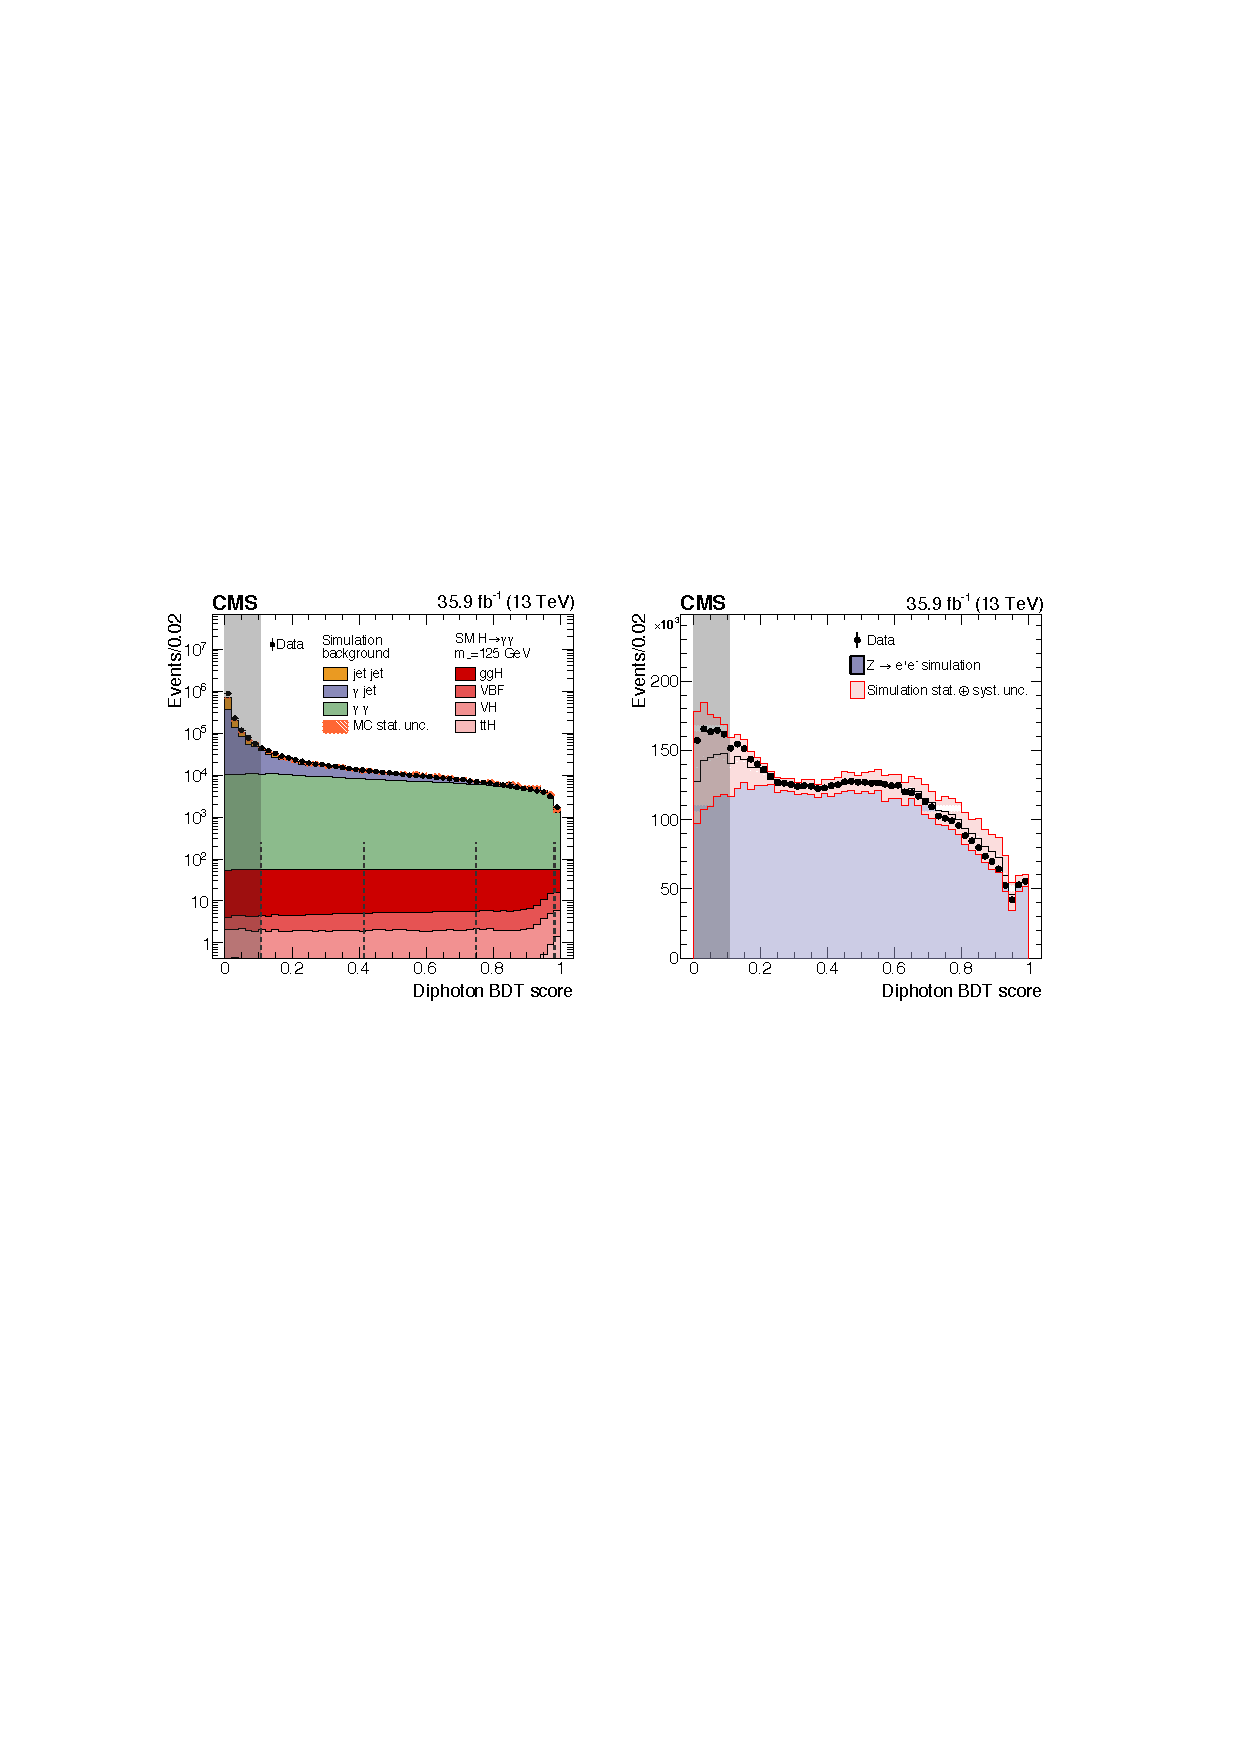
\includegraphics[width=0.99\textwidth]{figures/event_selection/diphoton_BDT.pdf}
    \end{center}
    \caption{Diphoton BDT score distributions for simulated signal, background, and data (left); and the \Zee control region (right). 
             A transformation has been applied to the score distribution such that the total signal distribution is flat.}
        \label{fig:event_categorisaton:diphoton_bdt}
\end{figure}


\subsection{Tagging Scheme}
Tagging is implemented as a fall-through sequence where diphotons are offered to each tag in order of priority (Table \ref{tab:event_categorisaton:tag_sequence}). 
If a diphoton is not accepted by a tag it then passes to the next tag for consideration until the final `untagged' tag category. 
If the diphoton does not meet the criteria for this last tag it is discarded.
In the case of multiple tagged candidate diphotons in an event we select the one with the highest priority tag and category, if they are in the same category we choose the diphoton with the highest diphoton $p_{T}$.

\begin{table}[h!]
    \begin{tabular}{ l || l | l}
        Tag & Target Process & Structure \\
        \hline
        \ttH Leptonic      & \ttH with semi-leptonic top decays & Single category \\
        \ttH Hadronic      & \ttH with fully-hadronic top decays & Single category \\
        ZH Leptonic        & VH with leptonically-decaying Z boson & Single category \\
        WH Leptonic        & VH with leptonically-decaying W boson & Single category \\
        VH Leptonic Loose  & VH with leptonically-decaying W or Z boson & Single category \\
        VBF                & VBF with dijet in the final state & Three categories \\
        VH MET            & VH with significant amount of \MET & Single category \\
        VH Hadronic        & VH with hadronically-decaying W or Z boson & Single category \\
        Untagged           & Inclusive & Four categories \\
    \end{tabular}
    \caption{The \Hgg tag sequence}
    \label{tab:event_categorisaton:tag_sequence}
\end{table}

In the remainder of this chapter we will describe each tag grouped by the production mode they target. In particular we will consider VBF tagging in detail and present a tag based on jet images and a dense CNN. 






\section{Top Fusion Tagging}
In the \ttH production mode, a top-antitop pair is produced in association with the Higgs boson. The top quark immediately decays to a b quark and a W boson which will subsequently decay leptonically or hadronically. In the former (semi-leptonic) case there will be a bottom quark jet plus an associated lepton with \MET from the W decay. In the latter (fully-hadronic) case there will be a bottom quark jet plus two quark jets from the W decay to quarks (Figure \ref{fig:event_categorisaton:top_decays}). 

\begin{figure}[h!]
    \begin{center}
        \begin{tikzpicture}[baseline=(current bounding box.center)]
        \begin{feynman}
            \vertex (a) {$t$};
            \vertex [right=of a] (b);
            \vertex [above right=of b] (f1);
            \vertex [below right=of b] (f2) {$b$};
            \vertex [above right=of f1] (f3) {$(u,c,t)$};
            \vertex [below right=of f1] (f4) {$(\bar{d},\bar{s},\bar{b})$};
            \diagram* {
                (a) -- [fermion] (b) -- [boson, edge label=\(W^{+}\)] (f1),
                (b) -- [fermion] (f2),
                (f1) -- [fermion] (f3),
                (f4) -- [fermion] (f1),
            };
        \end{feynman}
        \end{tikzpicture}
        %
        \qquad
        \begin{tikzpicture}[baseline=(current bounding box.center)]
        \begin{feynman}
            \vertex (a) {$t$};
            \vertex [right=of a] (b);
            \vertex [above right=of b] (f1);
            \vertex [below right=of b] (f2) {$b$};
            \vertex [above right=of f1] (f3) {${(\nu_{e},\nu_{\mu},\nu_{\tau})}$};
            \vertex [below right=of f1] (f4) {${(\bar{e},\bar{\mu},\bar{\tau})}$};
            \diagram* {
                (a) -- [fermion] (b) -- [boson, edge label=\(W^{+}\)] (f1),
                (b) -- [fermion] (f2),
                (f1) -- [fermion] (f3),
                (f4) -- [fermion] (f1),
            };
        \end{feynman}
        \end{tikzpicture}
    \end{center}
    \caption{Top quark decay modes: a fully-hadronic decay (left) and a semi-leptonic decay (right).}
    \label{fig:event_categorisaton:top_decays}
\end{figure}

The top tags target these two decay modes: the leptonic tag searches for \ttH events where at least one top quark decays semi-leptonically, and the hadronic tag searches for \ttH events where both top quarks decay fully-hadronically. 

\subsection{\ttH Leptonic}
This tag uses a set of selections on kinematic properties of leptons and jets in the event. 
Leptons are required to pass selection requirements depending on their flavour
\begin{itemize}[leftmargin=.5in,noitemsep]
    \item Diphoton BDT score $> 0.11$ 
    \item At least one selected lepton with $p_{T} > 20$\,GeV
    \item All selected leptons are required to have an angular separation from a signal photon of $R(\ell,\gamma) > 0.35$
    \item $|m_{e\gamma} - m_{Z}| > 5$\,GeV (electrons only)
    \item A minimum of two jets in the event with $p_{T} > 25$\,GeV, $|\eta| < 2.4$, $R(j,\gamma) > 0.4$ and $R(j,\ell) > 0.4$
    \item At least one jet is tagged as b jet by the CSV tagger (medium requirement)
\end{itemize}


\subsection{\ttH Hadronic}
This tag uses a set of selections on kinematic properties of the jets in the event, as well as a dedicated BDT. The \ttH hadronic BDT is trained on the following input features:
\begin{itemize}[leftmargin=.5in,noitemsep]
    \item the number of jets with $p_{T} > 25$\,GeV,
    \item the $p_{T}$ of the leading jet,
    \item the two highest scores of the CSV b-tagger.
\end{itemize}
A selection on the BDT output score (Figure \ref{fig:event_categorisaton:tth_hadronic_bdt}) is optimised simultaneously on simulation with a selection on the diphoton BDT score to maximise expected precision on the signal strength of the \ttH production channel. 

\begin{figure}[h!]
    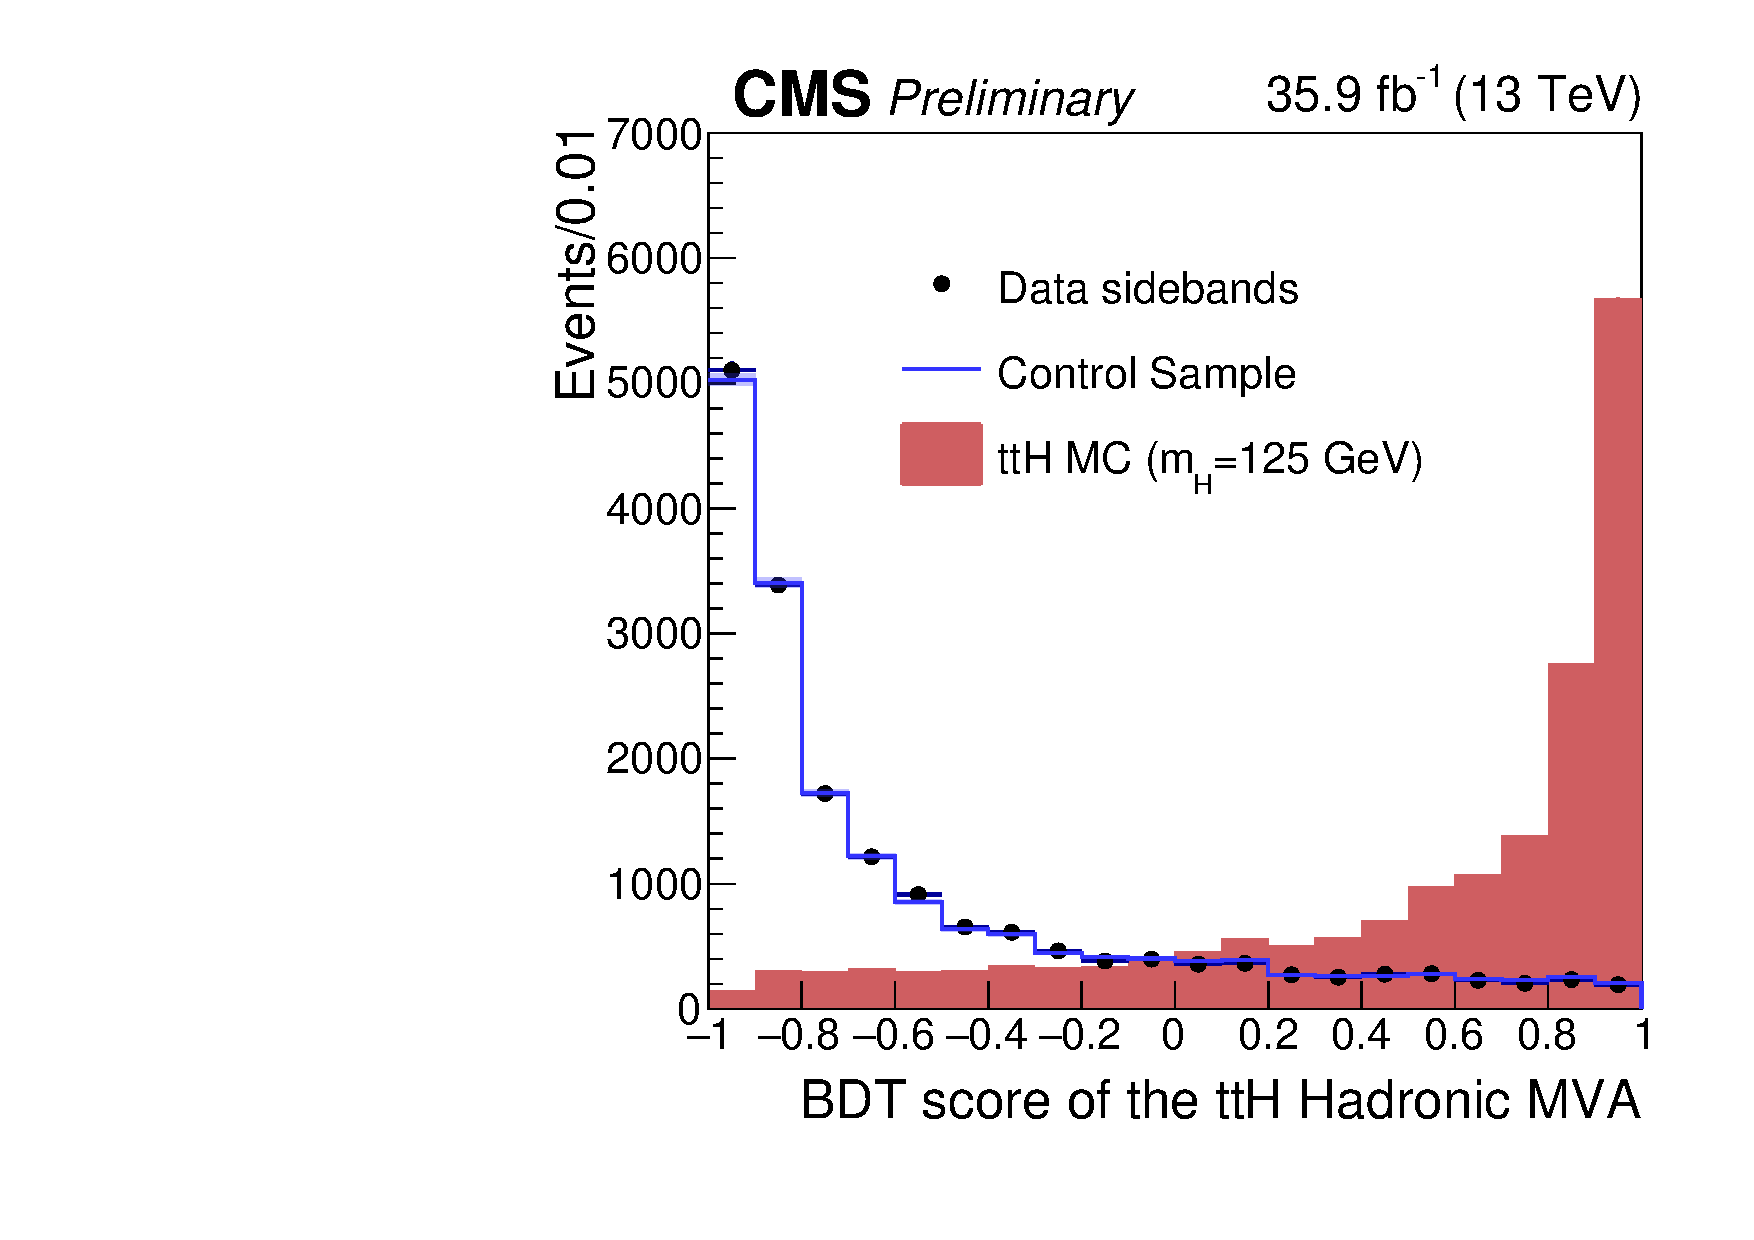
\includegraphics[width=0.49\textwidth]{figures/event_selection/Figure_006.pdf}
    \caption{Score distribution of the hadronic \ttH BDT. The blue lined histogram shows the distribution for the control region, the red filled histogram shows the score distribution for simulated signal, and the points show the score distribution of the data sideband regions ($m_{\gamma\gamma} < 115$\,GeV or $m_{\gamma\gamma} > 135$\,GeV).}
        \label{fig:event_categorisaton:tth_hadronic_bdt}
\end{figure}

A control region is constructed by selecting photon pairs where one passes the preselection and photon ID requirements, whilst the other has no preselection requirement and the photon ID is inverted.
These events are then weighted in $\eta$ and $p_T$ of the photons to reproduce the kinematic properties of the signal region.

The selection requirements of the \ttH Hadronic tag are as follows:
\begin{itemize}[leftmargin=.5in,noitemsep]
    \item $p_{T}/m_{\gamma\gamma} > 1/3$ and $1/4$ for leading and subleading photons respectively,
    \item diphoton BDT score $> 0.4$,
    \item no leptons that meet the criteria of the \ttH Leptonic tag
    \item a minimum of three jets in the event with $p_{T} > 25$\,GeV and $|\eta| < 2.4$,
    \item at least one jet is tagged as b jet by the CSV tagger (medium requirement),
    \item a \ttH Hadronic BDT score above 0.75.
\end{itemize}



\section{Associated Production Tagging}
In the associated production (VH) mode a W or Z is produced in association with the Higgs boson. The VH tags target different vector bosons decaying in different ways which can manifest as leptons, jets or \MET in the event.
All of the leptonic VH tags are selection-based and have various isolation requirements to avoid contamination from Drell-Yan background processes.

\subsection{ZH Leptonic}
Targets Higgs production in association with a Z boson that subsequently decays leptonically with stringent requirements. The selection criteria are as follows:
\begin{itemize}[leftmargin=.5in,noitemsep]
    \item $p_{T}/m_{\gamma\gamma} > 3/8$ and $1/4$ for leading and subleading photons respectively,
    \item diphoton BDT score $> 0.11$,
    \item two same-flavour leptons with $p_T > 20$\,GeV and satisfying the same requirements as in the \ttH Leptonic tag
    \item $70 < m_{\ell\ell} < 110$\,GeV,
    \item $R(\gamma,e) > 1.0$, or $R(\gamma,\mu) > 0.5$,
    \item conversion electron veto: if an electron and a photon share a supercluser, the electron track must be well-separated from the supercluser centre ($R(SC,e_{\mathrm{track}}) > 0.4$).
\end{itemize}


\subsection{WH Leptonic}
Targets Higgs production in association with a W$^{\pm}$ boson that subsequently decays leptonically with stringent requirements. The selection criteria are as follows:
\begin{itemize}[leftmargin=.5in,noitemsep]
    \item $p_{T}/m_{\gamma\gamma} > 3/8$ and $1/4$ for leading and subleading photons respectively,
    \item diphoton BDT score $> 0.28$,
    \item at minimum one lepton with $p_T > 20$\,GeV and satisfying the same requirements as in the \ttH Leptonic tag
    \item $R(\gamma,\ell) > 1.0$,
    \item \MET$> 45$\,GeV,
    \item a maximum of two jets each satisfying $p_T > 20$\,GeV, $|\eta| < 2.4$, $R(j,\ell) > 0.4$, $R(j,\gamma) > 0.4$,
    \item electron conversion veto as in the ZH Leptonic tag
\end{itemize}



\subsection{VH Leptonic Loose}
Targets Higgs production in association with either W$^{\pm}$ or Z which then decay leptonically. This tag uses a looser \MET selection of \MET$ < 45$\, GeV, with the rest of the selection being the same as WH Leptonic.

\subsection{VH MET}
Targets Higgs associated production with \MET from at least one missing lepton. The selection criteria are as follows:
\begin{itemize}[leftmargin=.5in,noitemsep]
    \item $p_{T}/m_{\gamma\gamma} > 3/8$ and $1/4$ for leading and subleading photons respectively,
    \item diphoton BDT score $> 0.79$,
    \item \MET$> 85$\,GeV,
    \item $|\Delta\phi(\gamma\gamma,E_{T}^{miss})| > 2.4$
\end{itemize}


\subsection{VH Hadronic}
Targets Higgs production in association with a W or Z boson that decays hadronically. The selection criteria are as follows:
\begin{itemize}[leftmargin=.5in,noitemsep]
    \item $p_{T}/m_{\gamma\gamma} > 1/2$ and $1/4$ for leading and subleading photons respectively, 
    \item diphoton BDT score $> 0.79$,
    \item a minimum of two jets with $p_T > 40$\,GeV and $|\eta| < 2.4$, $R(j,\gamma) > 0.4$,
    \item dijet invariant mass $60 < m_{jj} < 120$\,GeV,
    \item $|\mathrm{cos}{\theta^{*}}|$
\end{itemize}













\section{VBF Tag}
The VBF production mode is characterised by its distinctive event topology and kinematics: two high-$p_{T}$ jets with large pseudorapidity separation and high invariant mass. Furthermore, the dijet substructure will also be distinctive with both jets originating from quarks, having colour connection to the proton remnant and possibly having correlations in structure between the two jets. 

Other production modes can also produce a Higgs boson in association with jets to produce a VBF-like final state. 
In particular, ggH can be a significant source of false positives due to its larger cross section and capacity to produce jets at next-to-leading order and from gluons radiating from the top loop. 

VBF tagging targets the VBF production mode by exploiting the distinctive properties of VBF dijets. In this chapter we will explore two approaches:
\begin{itemize}[leftmargin=.5in,noitemsep]
    \item A tag based on two BDTs with engineered kinematic features. This is the approach used in the 2016 \Hgg analysis. 
    \item A tag based on a single dense convolutional neural network that receives jet structure information in the form of images in addition to engineered kinematic features. 
\end{itemize}
Both tags use the same event preselection, and produce scores used to define event categories which enhance the expected significance of the VBF channel and will be evaluated in the same way. The only difference will be the machine learning model that the tags are based around, and the extra image-based information in the dense CNN tag.  
%Figure of merit
The measure of significance used as a figure of merit when developing the VBF tag is the approximate mean significance (AMS) introduced in the Higgs ML challenge (ref),
\begin{equation}
    \mathrm{AMS}_{2} = \sqrt{2\left( (s+b+b_{\mathrm{reg}})\log\left(1 + \frac{s}{b+b_{\mathrm{reg}}}\right) - s \right)}.
\end{equation}
Where $s$ is the total number of signal events, $b$ is the total number of background events, and $b_{\mathrm{reg}}$ is a regularisation term that reduces sensitivity to local optima. 
This is calculated by simulatneously fitting an exponential plus a double Gaussian function to the diphoton mass distribution. The background and signal event weights from an interval of two effective standard deviations around the peak are summed to produce $s$ and $b$, and to estimate $\mathrm{AMS}_{2}$. 

The classifiers themselves are evaluated using area under the `Receiver Operating Characteristic' curve (AUROC) which is a measure of the performance of a binary classifier that is unaffected by large class imballance. The final models produce a score which is then used to define categories which maximise $\mathrm{AMS}_{2}$.







\subsection{Selections}

When a candidate diphoton is considered for VBF selection we apply additional requirements based on the jet content of the event. First requirements are applied on a per-jet basis, if there are more than two jets which meet these requirements the top two in $p_{T}$ are selected to form a dijet. Finally, a preselection based on dijet kinematics is applied the candate dijet. If it does not pass the event falls through to the untagged categories. 

\subsubsection{Jet Selection}

Jets are required to meet the criteria detailed in the previous chapter plus additional requirements based on pileup jet identification (PUJID) and pseudorapidity ($|\eta_{j}| < 4.7$).
PUJID uses a BDT classifier \ref{CMS-PAS-JME-13-005} that takes a collection of jet shape variables and produces a score for each jet. A collection of selections on this score are then applied for bins in $p_{T}$ and $\eta$ (Table \ref{tab:event_selection:tight_pujid}). In this analysis the tight working point is used as this gives the highest exptected significance for the VBF tag, and also leads to marked improvement in data/simulation agreement in $\eta$ in the \Zee plus jets control region.% \ref{fig:event_categorisaton:sublead_eta_pujid}. 
\begin{table}[h!]
    \begin{tabular}{ l || c | c | c | c }
         & $|\eta| < 2.5$ & $2.5 \leq |\eta| < 2.75$ & $2.75 \leq |\eta| < 3.0$ & $3.0 \leq |\eta| < 5.0$ \\
        \hline
        \hline
        $20 < p_{T} \leq 30$  & $0.69$ & $-0.35$ & $-0.26$ & $-0.21$ \\
        $30 < p_{T} \leq 50$  & $0.86$ & $-0.1$  & $-0.05$ & $-0.01$ \\
        $50 < p_{T} \leq 100$ & $0.95$ & $0.28$  & $0.31$  & $0.28$  \\
\end{tabular}
    \caption{Pileup jet ID cuts of the tight working point}
    \label{tab:event_selection:tight_pujid}
\end{table}

%\begin{figure}[h!]
%    \begin{center}
%        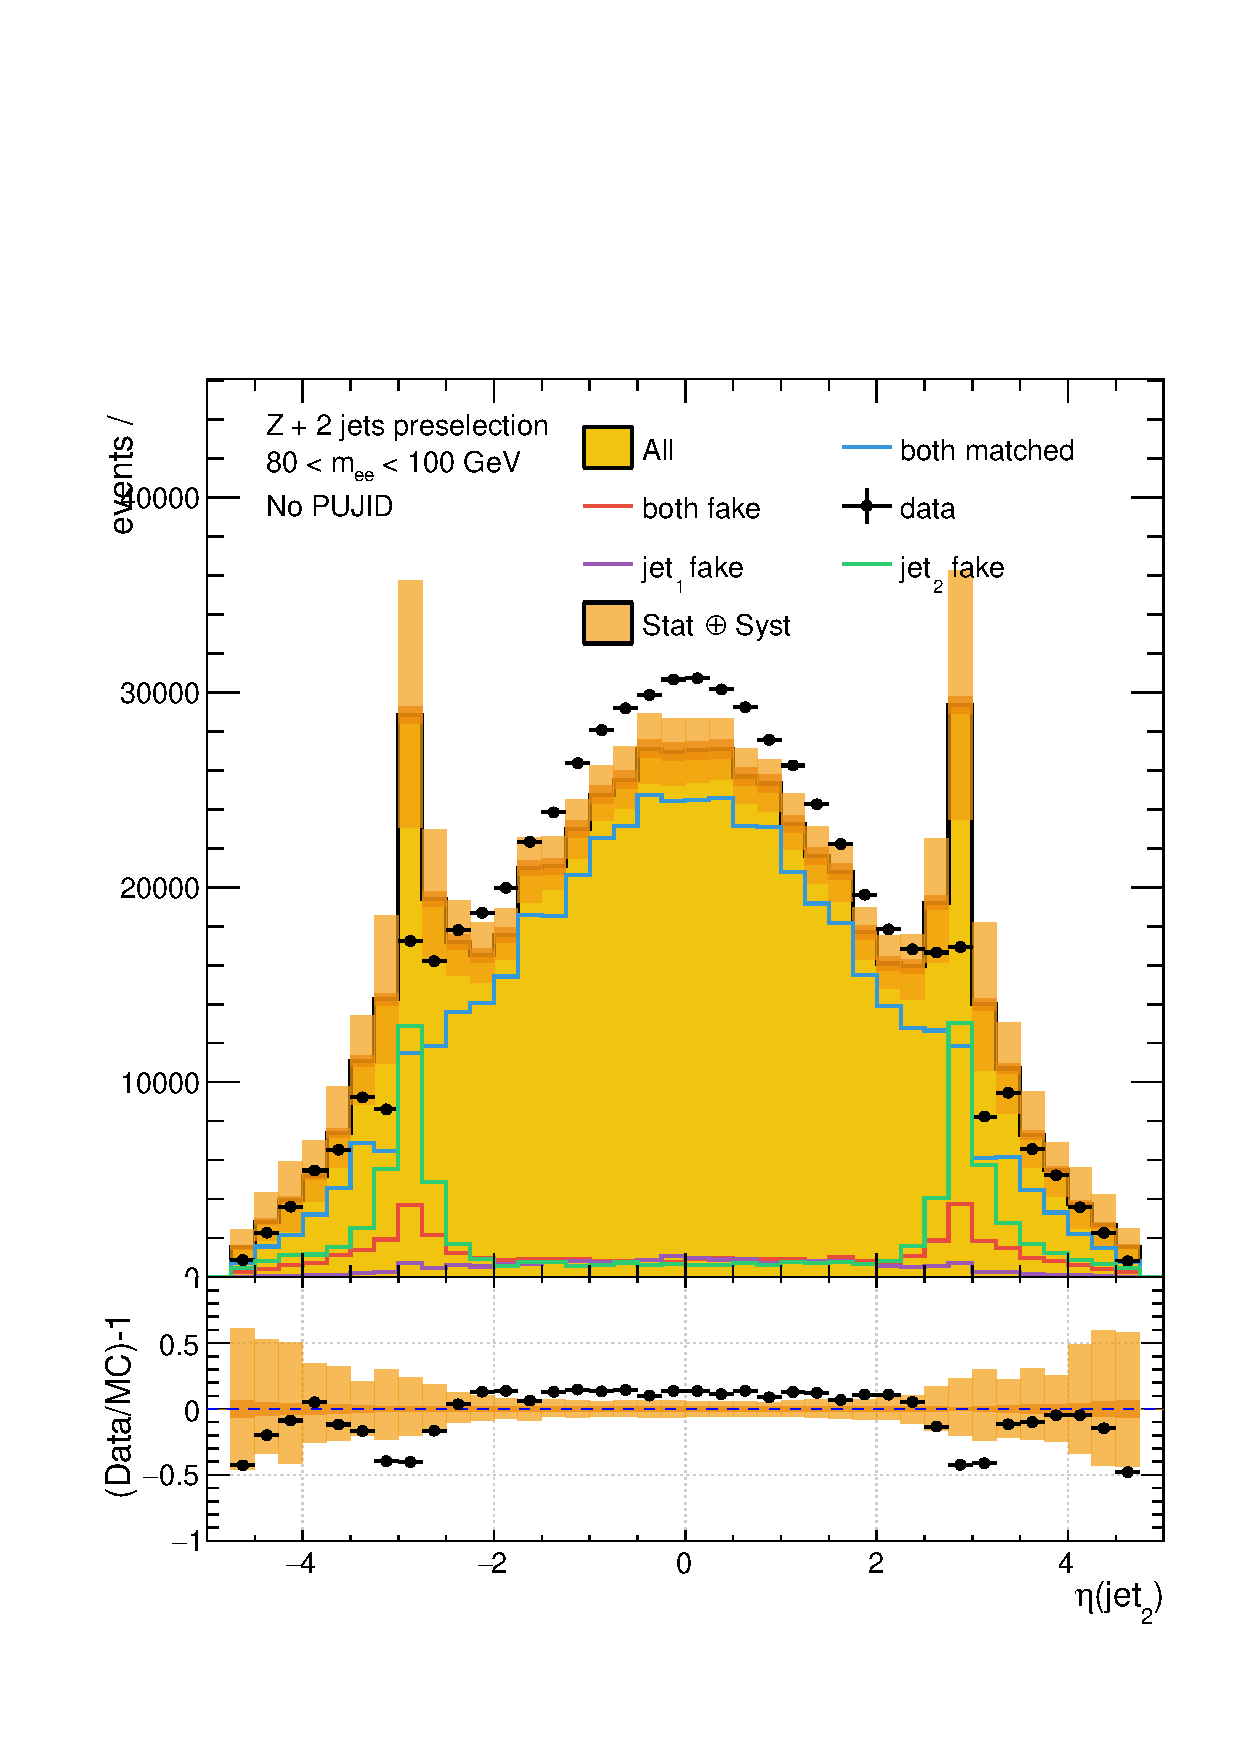
\includegraphics[width=0.45\textwidth]{figures/event_selection/stack_histogram_dijet_subleadEta_zplus2j_none_inclusive_.pdf}
%        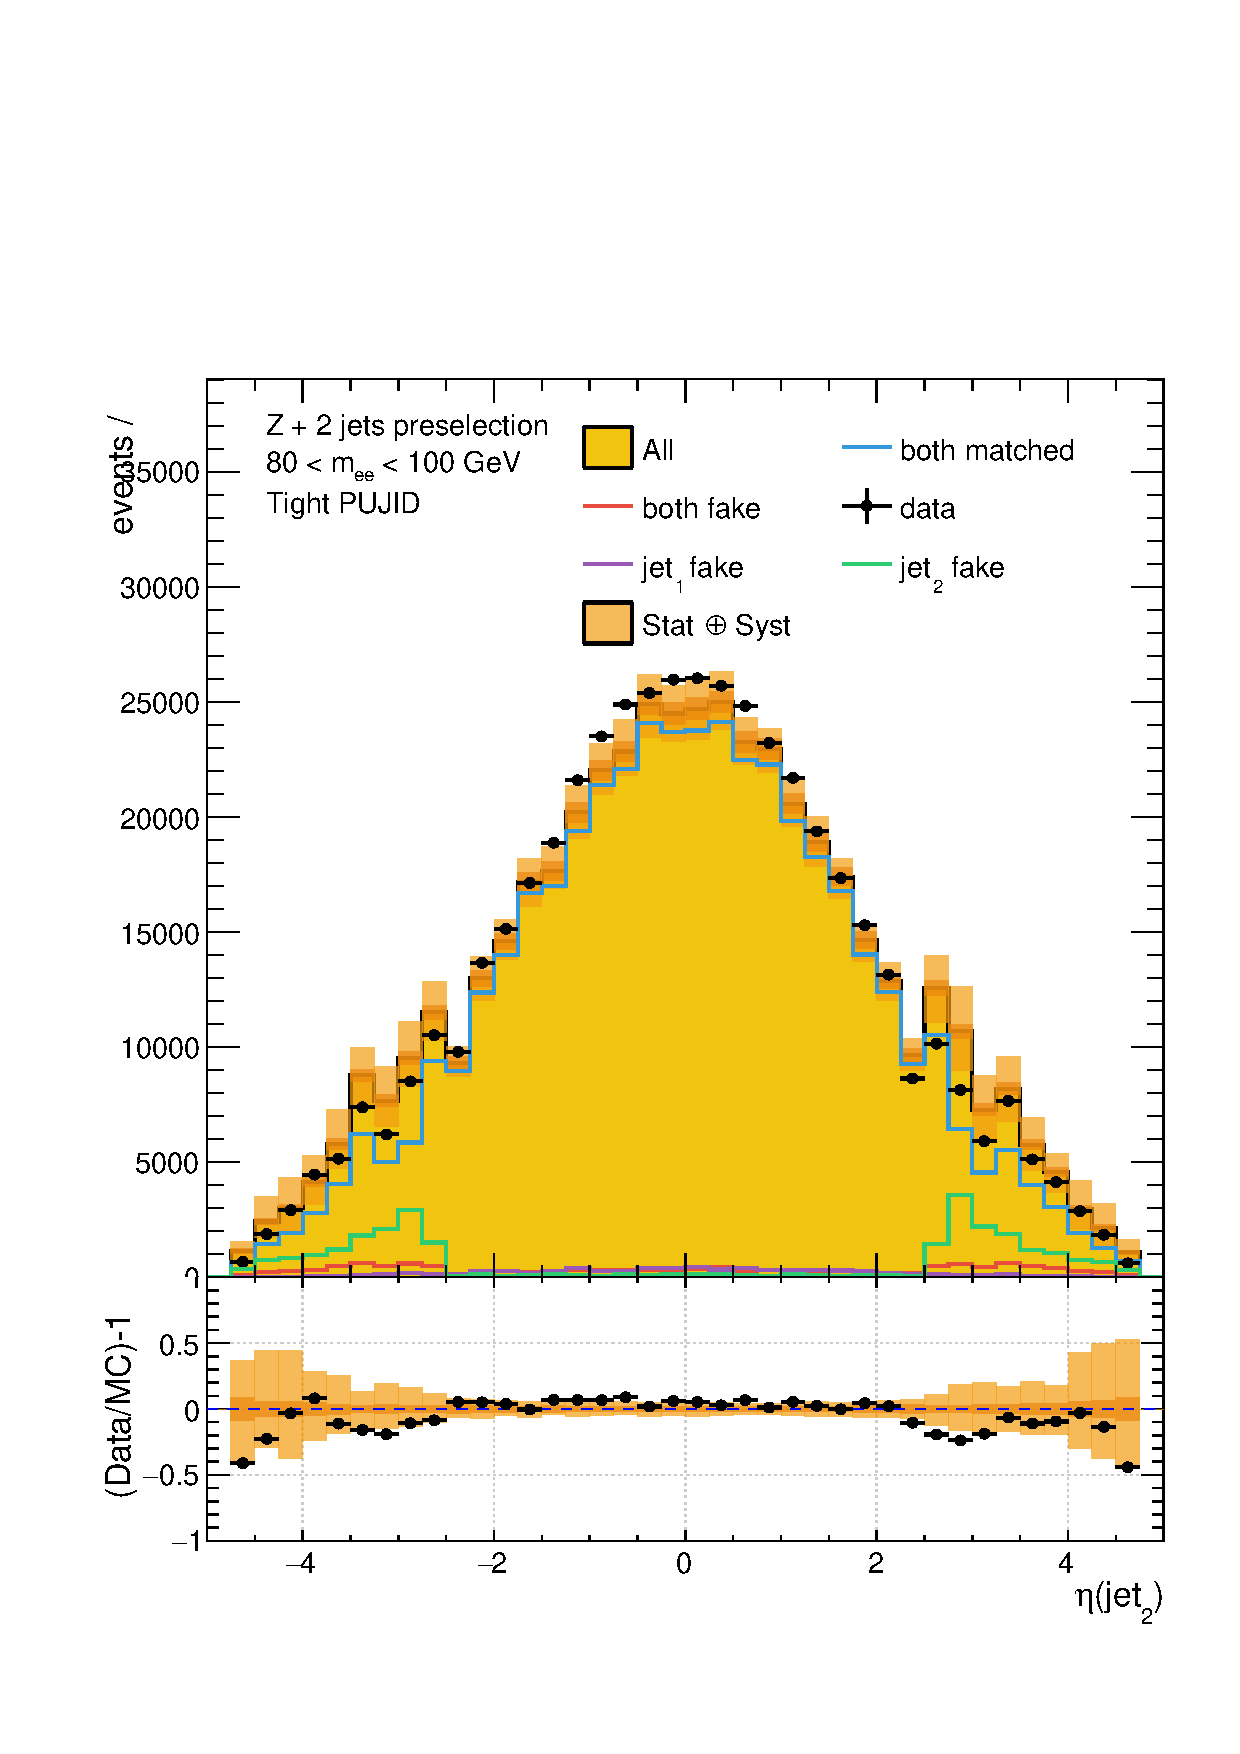
\includegraphics[width=0.45\textwidth]{figures/event_selection/stack_histogram_dijet_subleadEta_zplus2j_tight_inclusive_.pdf}
%    \end{center}
%    \caption{Sublead pseudorapidity for no PUJID and the tight working point. We note a substantial decrease in fake jets from the endcap/hadronic forward transition region around $|\eta|=3$, and an overall improvement in agreement between simulation and data.}
%    \label{fig:event_categorisaton:sublead_eta_pujid}
%\end{figure}







\subsubsection{Dijet Preselection}
Dijets are formed by selecting the two highest-$p_T$ jets in the event which pass the jet selection requirements. The highest-$p_T$ jet in the pair is referred to as the leadning jet, and the other jet as the subleading jet. If there are fewer than two jets the event is rejected by the VBF tag and falls through to untagged. 
Candidate dijets are required to meet the following selection before being presented to the machine learning model:
\begin{itemize}[leftmargin=.5in,noitemsep]
    \item $p_{T}/m_{\gamma\gamma} > 1/3$ and $1/4$ for leading and subleading photon respectively,
    \item photon ID BDT score $> -0.2$ for both photons,
    \item dijet invariant mass $m_{jj} > 250$\,GeV,
    \item jet $p_{T} > 40$\,GeV and $> 30$\,GeV for the leading and subleading jets respectively,
%    \item absolute pseudorapidity $|\eta| < 4.7$ for both jets.
\end{itemize}

The requirement on photon ID score is to mitigate a particular problem with the diphoton BDT. Certain background events where the diphoton has a high $p_T$ are assigned a high score even when they have a low photon ID score. This is occuring because the diphoton BDT is trained over all Higgs production channels and the VBF channel is a smaller (lower-weighted due to its cross section) proportion of the signal it is targeting. A high-$p_T$ diphoton is strongly indicative of ggH when there are no additional jets, but in the VBF phase space background diphotons can have a higher-$p_T$ due to the recoiling jets. The diphoton BDT therefore underperforms in the VBF phase space, but some of these events can be removed due to their low photon ID score. 









\subsection{Dijet BDT}
The dijet BDT is the first of the two BDTs in the 2016 VBF tag structure. 
Its purpose is to evaluate how VBF-like events are based on kinematic information from the dijet and the diphoton, and in particular to handle the rejection of ggH.
The BDT receives the following features which are chosen to minimise correlation with the diphoton mass:
\begin{itemize}[leftmargin=.5in,noitemsep]
    \item $p_{T}/m_{\gamma\gamma}$ for the leading and subleading photons
    \item $p_{T}^{j1}$ and $p_{T}^{j2}$, the transverse momenta of the leading and subleading jets respectively
    \item $m_{jj}$ the invariant mass of the dijet
    \item $\Delta\eta$ the pseudorapidity gap between the two jets
    \item $\mathrm{min}\Delta{R}(\gamma,j)$ the smallest angular separation between either of the diphoton photons and either of the dijet jets
    \item $|\Delta\phi_{\gamma\gamma{jj}}|$ the absolute azimuthal angular difference between the diphoton and dijet
    \item $|\Delta\phi_{jj}|$ the absolute azimuthal angular difference between the jets of the dijet
    \item $C_{\gamma\gamma}$ the diphoton centrality expressed as:
        \begin{equation}
            C_{\gamma\gamma} = \mathrm{exp}\left(-\frac{4}{(\eta_{j1} - \eta_{j2})^{2}}\left( \eta_{\gamma\gamma} - \frac{\eta_{j1} + \eta_{j2}}{2} \right)^{2}\right)
        \end{equation}
        where $\eta_{j1}$ and $\eta_{j2}$ are the pseudorapidities of the leading and subleading jets.
\end{itemize}
Their distributions with the VBF preselection applied are shown in Figure \ref{fig:event_categorisaton:dijet_bdt_features}.
This dijet BDT is trained on all simulated SM background samples with ggH included versus VBF. To increase the number of training examples we train with a loosened dijet preselection requirement where the $p_{T}^{\gamma}/m_{\gamma\gamma}$ are reduced to $1/4$ and $1/5$, the jet $p_T$ cuts are reduced by 10\,GeV, the dijet invariant mass cut is reduced to 100\,GeV.
\begin{figure}[h!]
    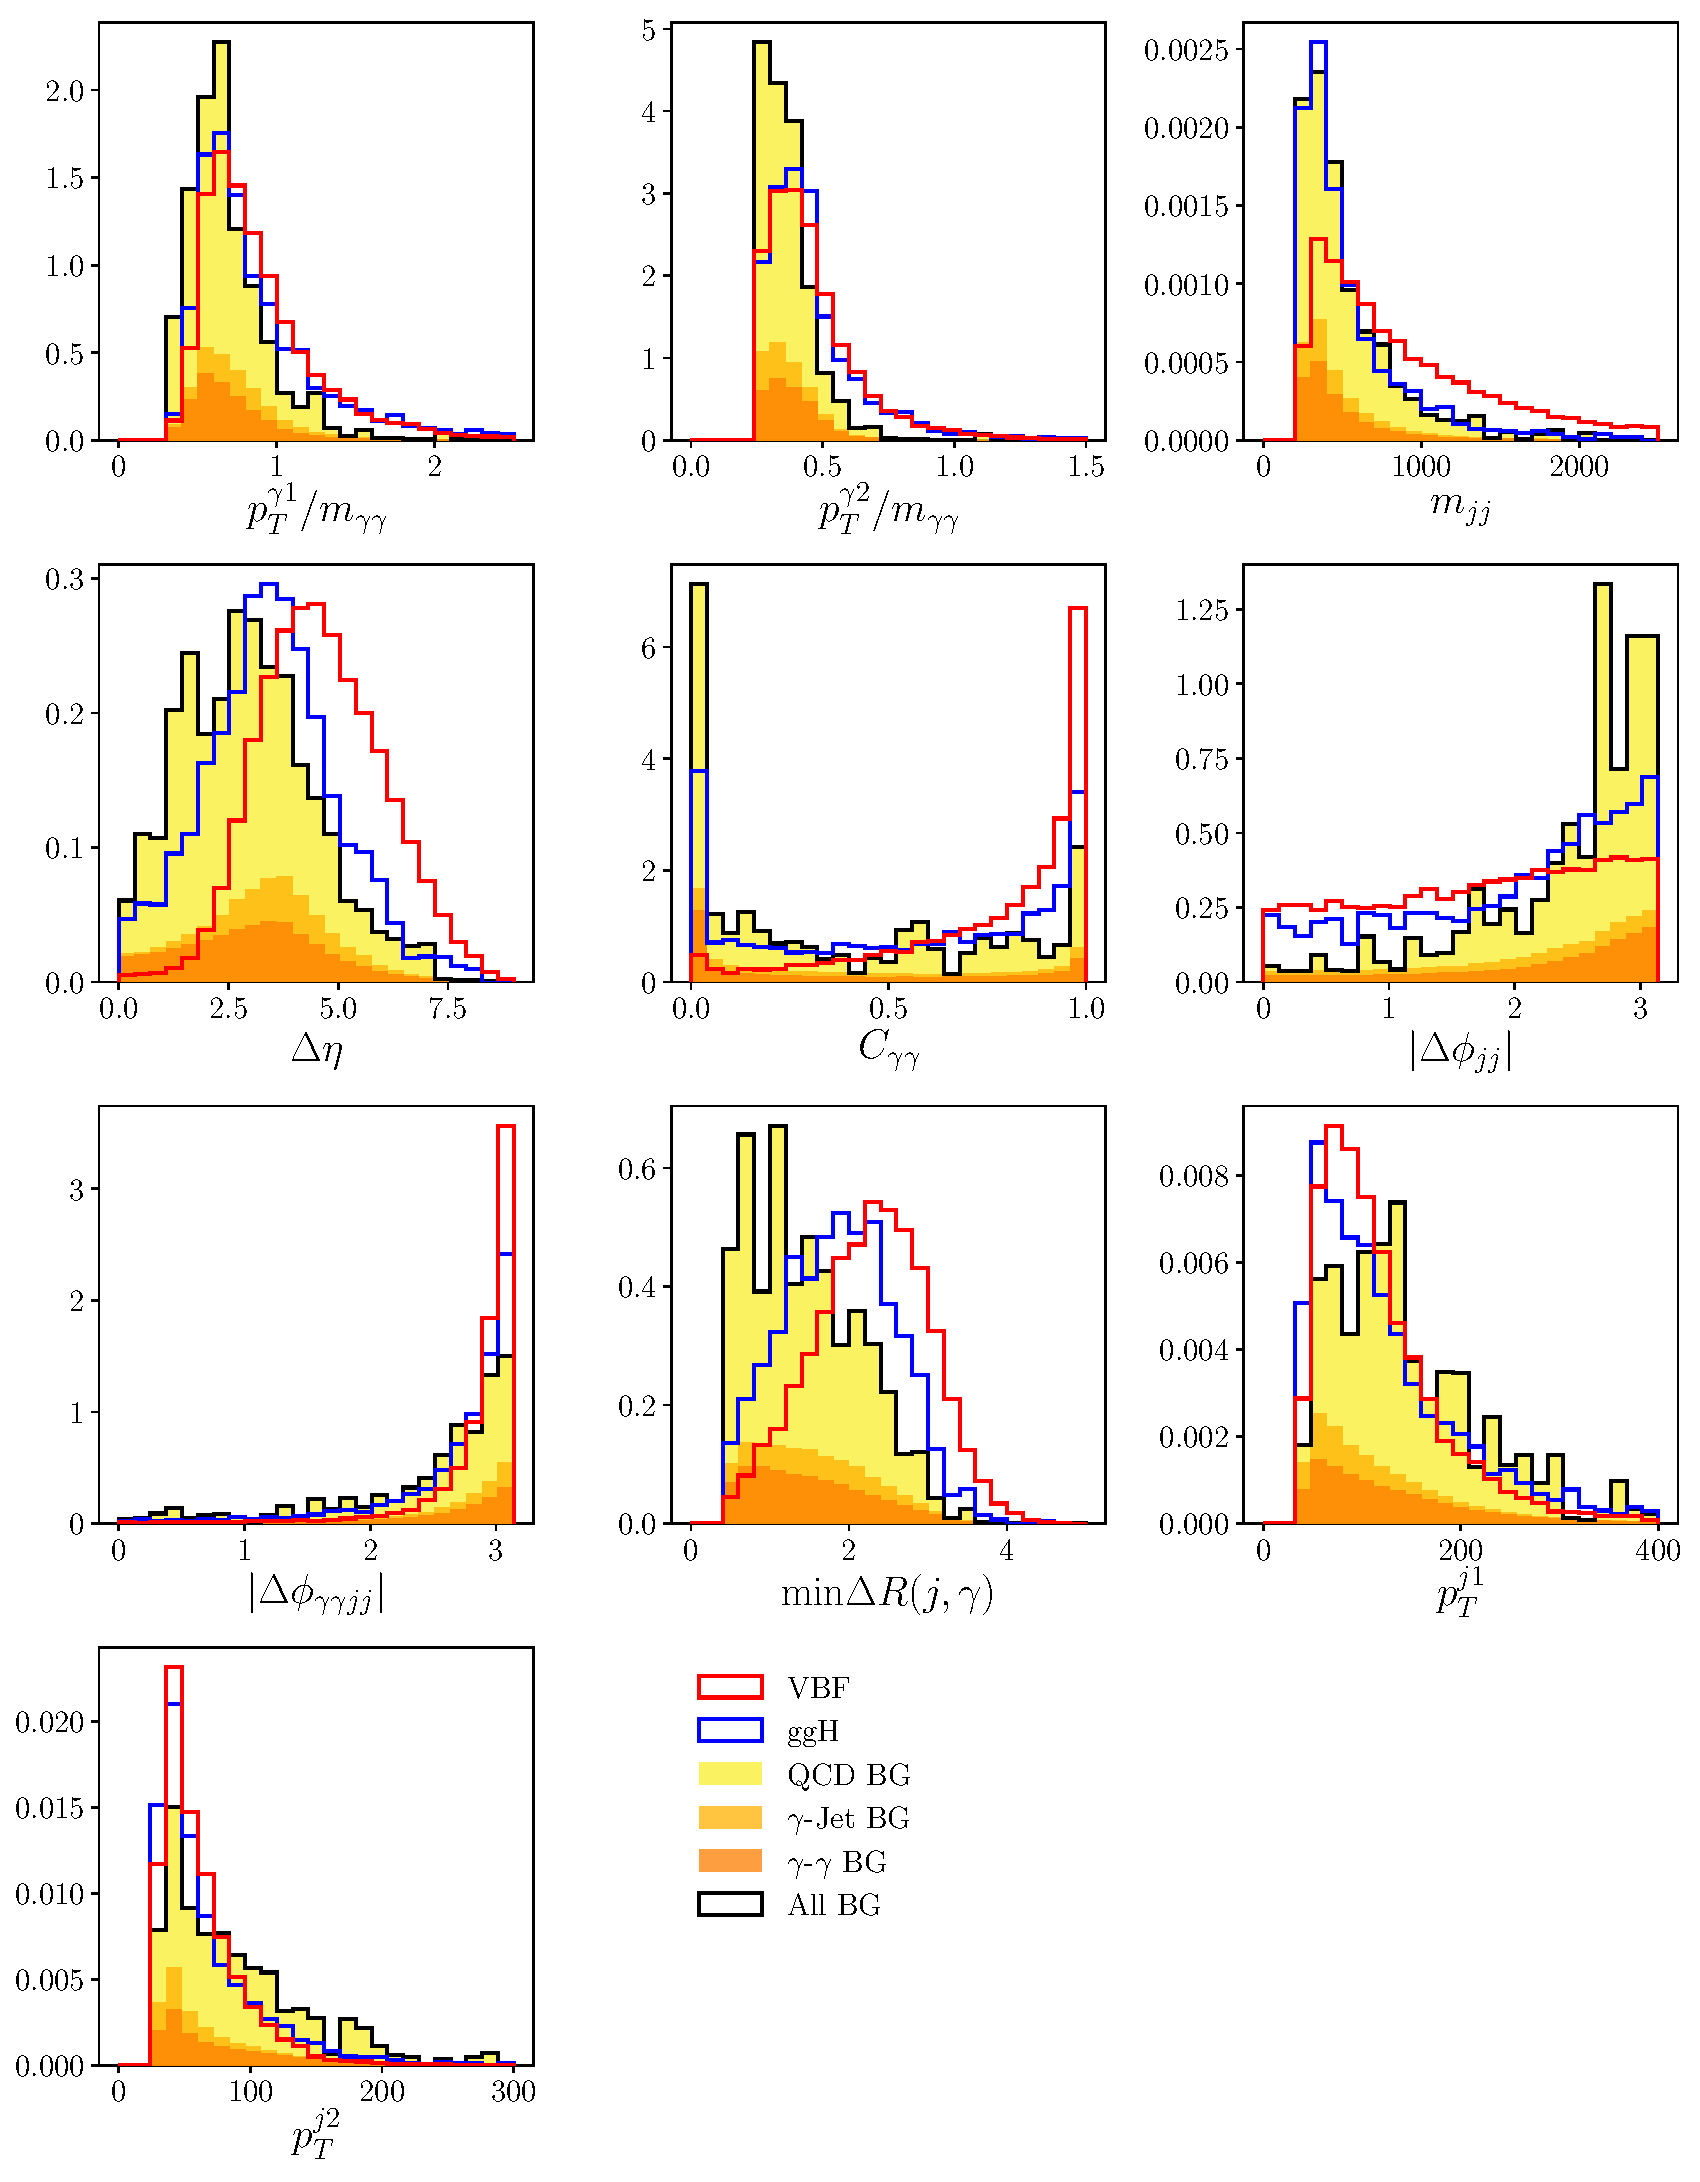
\includegraphics[width=0.98\textwidth]{figures/event_selection/dijet_BDT_features_splitBG_PS.pdf}
    \caption{Dijet BDT feature distributions with the full VBF preselection. Distributions are all normalised to unity with solid red corresponding to VBF, blue line to ggH, and black line to SM background}
    \label{fig:event_categorisaton:dijet_bdt_features}
\end{figure}

The normalised score distributions for the classes and the ROC curves for each individual sample are shown in Figure \ref{fig:event_categorisaton:dijet_bdt_performance}.
These scores are then used as an input feature in the next BDT in the VBF tag: the combined BDT. 

\begin{figure}[h!]
        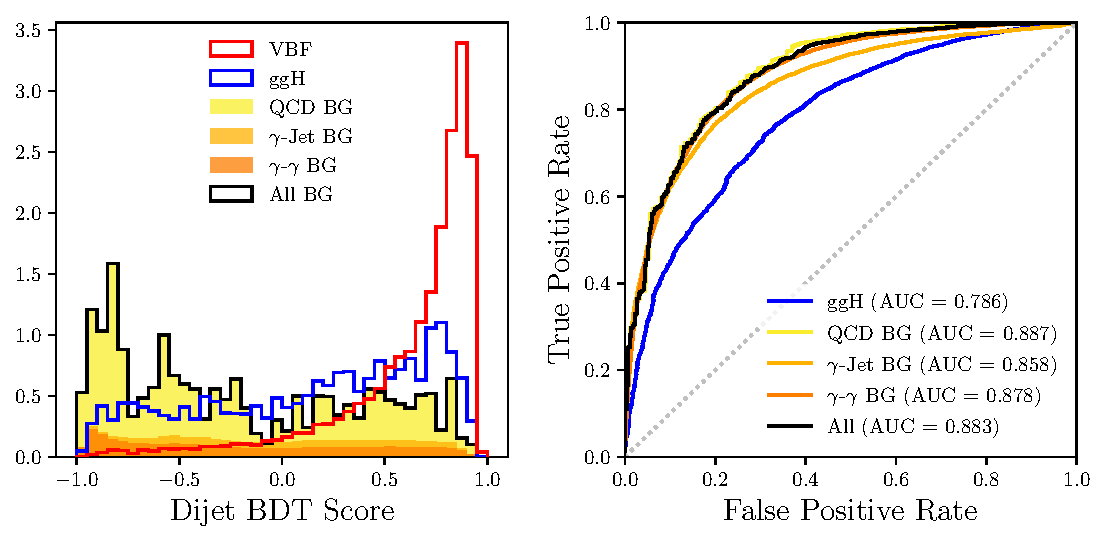
\includegraphics[width=0.75\textwidth]{figures/event_selection/dijet_BDT_PS.pdf}
    \caption{Dijet BDT performance. On the left are the output score distributions for VBF (red), ggH (blue) and SM background (black). On the right are the ROC curves for the dijet BDT split into the different samples. We note that the performance against ggH is lower than the other backgrounds.}
    \label{fig:event_categorisaton:dijet_bdt_performance}
\end{figure}









\subsection{Combined BDT}
The purpose of the combined BDT is to combine information from the diphoton BDT, and dijet BDT to produce the final discriminant score for defining VBF tag categories. 
Specifically, it takes the following input features
\begin{itemize}[leftmargin=.5in,noitemsep]
    \item diphoton BDT score
    \item dijet BDT score
    \item $p_{T}^{\gamma\gamma}/m_{\gamma\gamma}$, the mass-scaled transverse momentum of the diphoton
\end{itemize}
The distributions of these features with the full VBF preselection applied are shown in Figure \ref{fig:event_categorisaton:combined_bdt_features}.
\begin{figure}[h!]
    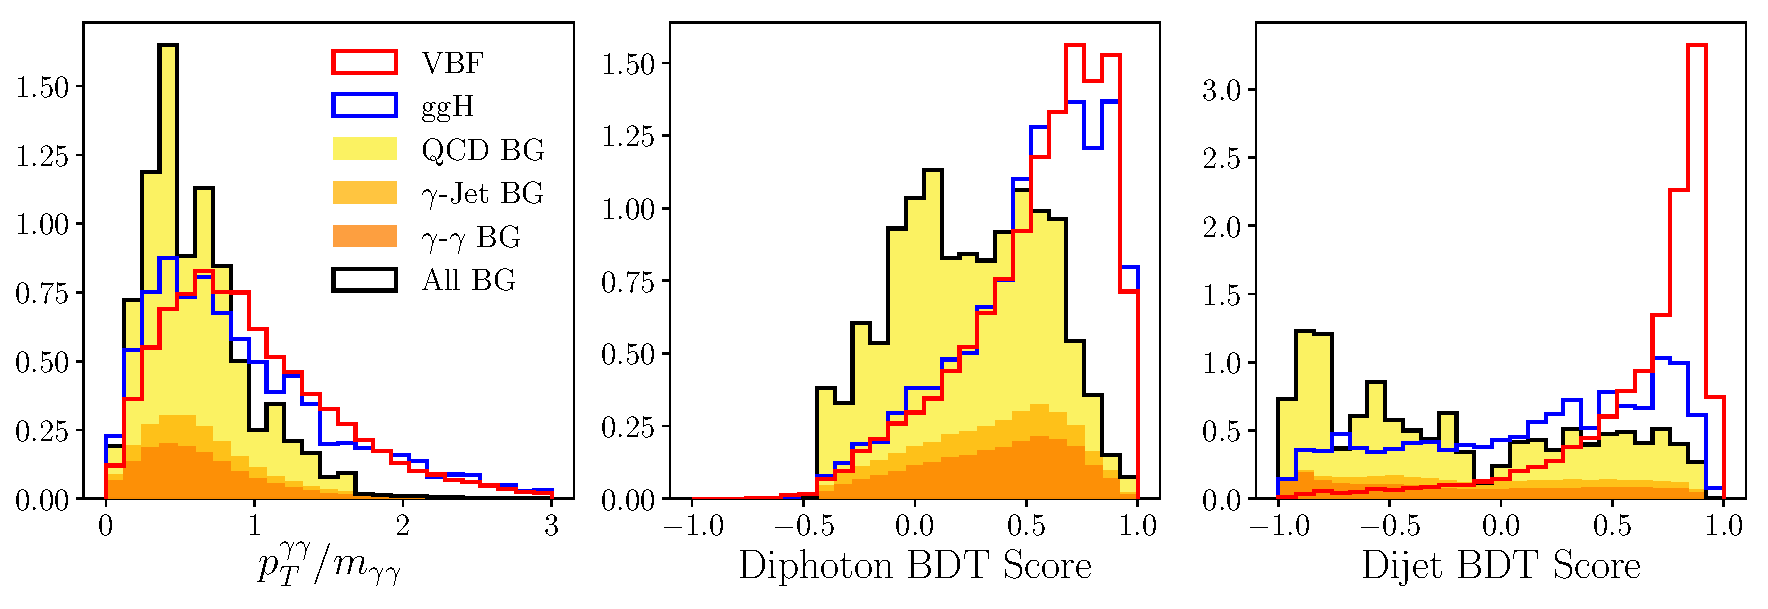
\includegraphics[width=0.98\textwidth]{figures/event_selection/combined_BDT_features_splitBG_PS.pdf}
    \caption{Combined BDT feature distributions with the full VBF preselection. Distributions are all normalised to unity with solid red corresponding to VBF, blue line to ggH, and black line to SM background}
    \label{fig:event_categorisaton:combined_bdt_features}
\end{figure}

The combined BDT is then trained with the SM background samples vs VBF. Gluon fusion is not included in this training as it is found to reduce the ability of this BDT to reject SM background, which is considered to be a higher priority than ggH rejection. 

The normalised combined score distributions for the classes and the ROC curves for each individual sample are shown in Figure \ref{fig:event_categorisaton:combined_bdt_performance}.
\begin{figure}[h!]
    \begin{center}
        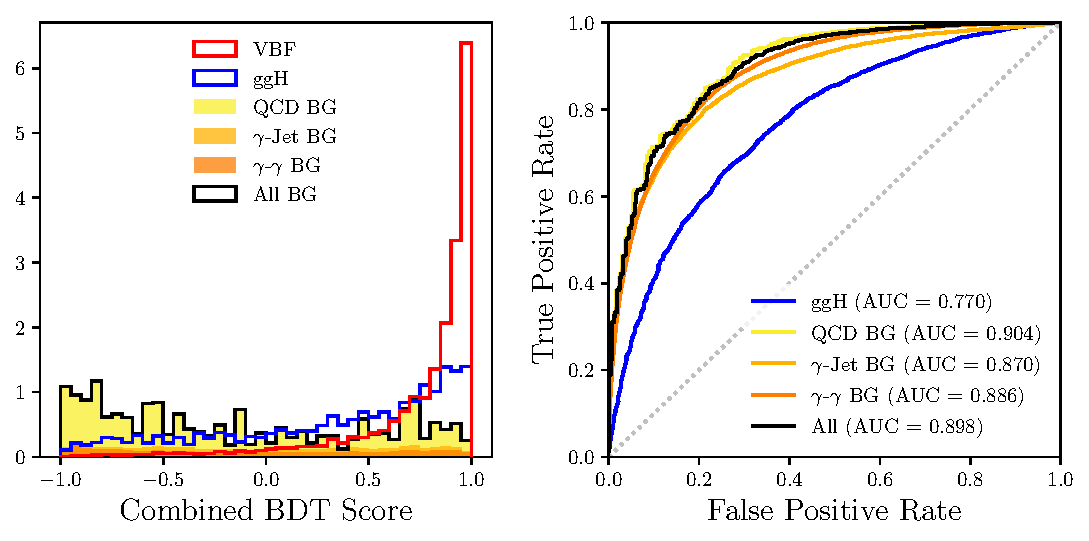
\includegraphics[width=0.75\textwidth]{figures/event_selection/combined_BDT_PS.pdf}
    \end{center}
    \caption{Combined BDT score distribution with the full VBF preselection. Distributions are all normalised to unity with solid red corresponding to VBF, blue line to ggH, and black line to SM background}
    \label{fig:event_categorisaton:combined_bdt_performance}
\end{figure}


Interpretation of the VBF tag goes in here?
\begin{figure}[h!]
    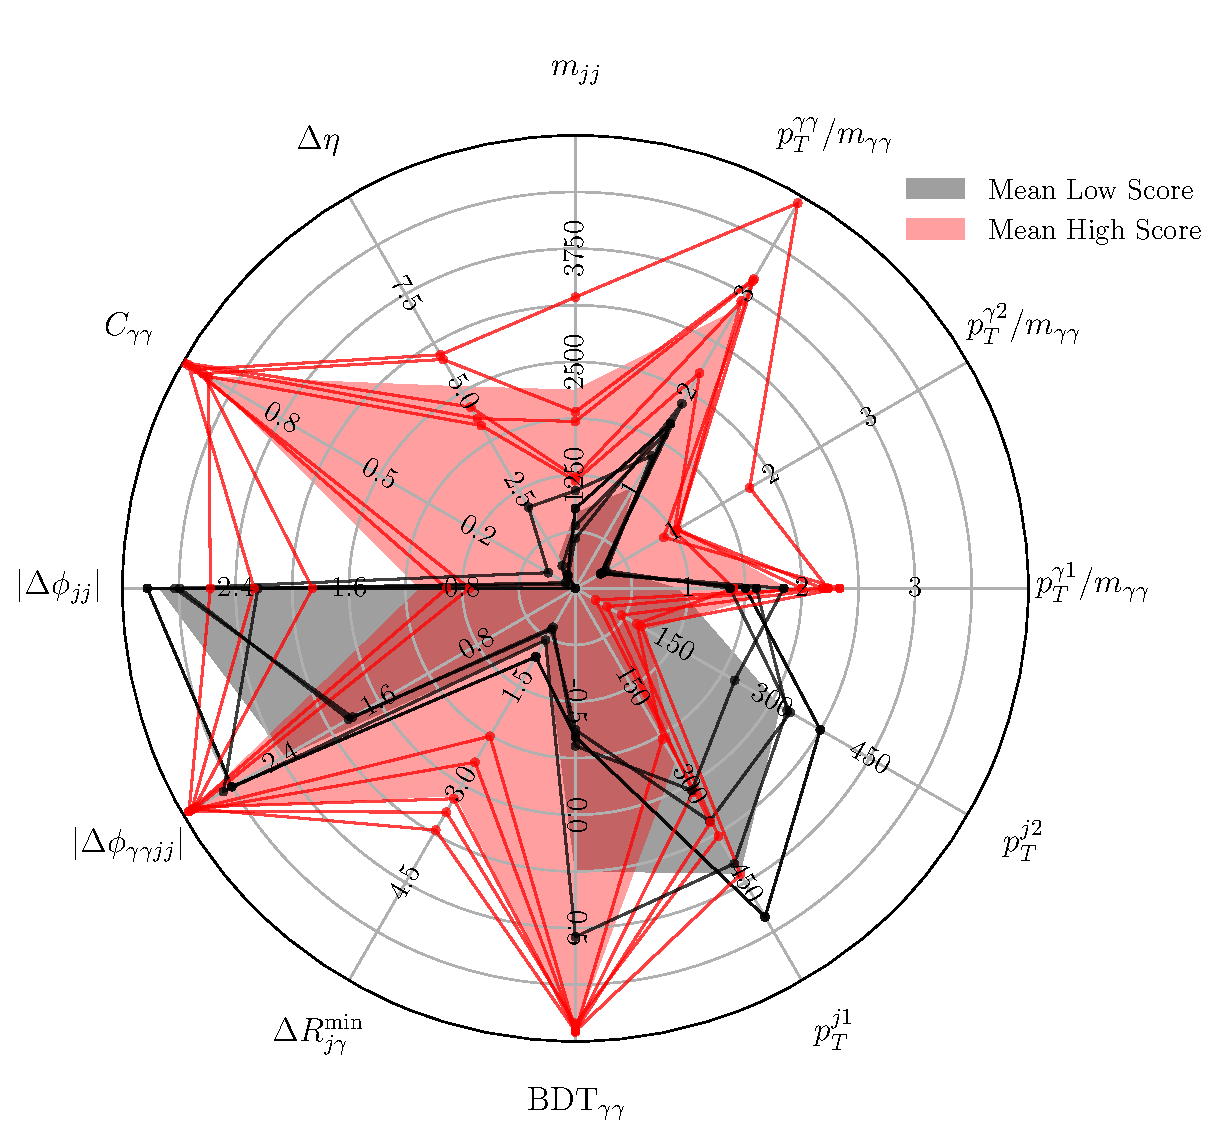
\includegraphics[width=0.75\textwidth]{figures/event_selection/eng_feature_radar_BDT.pdf}
    \caption{BDT high and low score events}
    \label{fig:event_categorisaton:bdt_based_vbf_tag_interpretation}
\end{figure}








\subsection{Categorisation}
Once an event is evaluated with the combined BDT and assigned a score, it is considered for inclusion in one of the VBF tag subcategories.
These categories are defined as requirements on the combined BDT score and are chosen such that they maximise the overall significance ($\mathrm{AMS}_2$).

Category boundaries are chosen by an optimisation procedure where the categories are varied simultaneously to find the set of values which 

\begin{figure}[h!]
    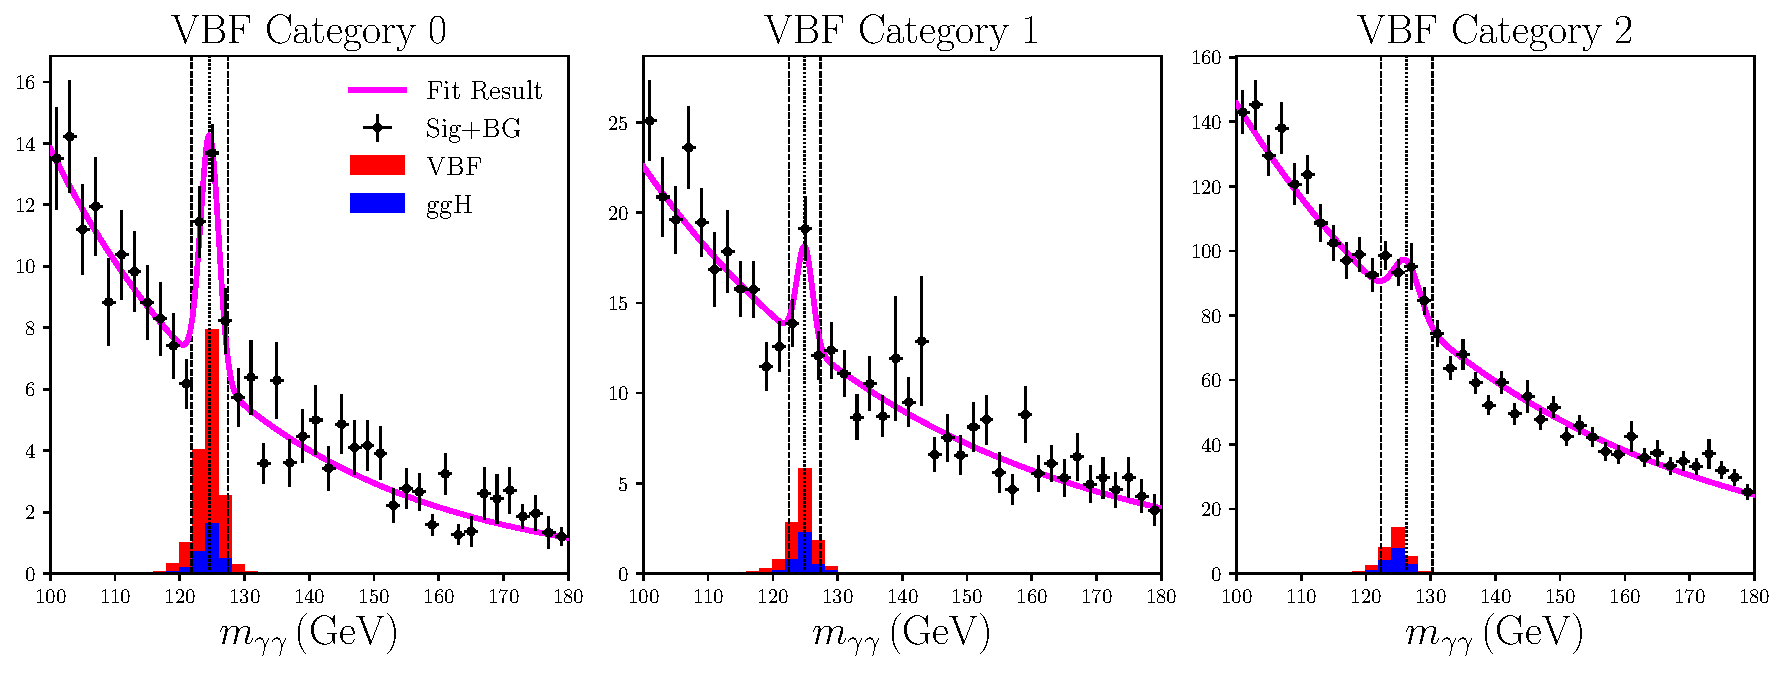
\includegraphics[width=1.0\textwidth]{figures/event_selection/BDT_mass_fits.pdf}
    \caption{Mass fits for estimating AMS$_2$}
    \label{fig:event_categorisaton:bdt_mass_fits}
\end{figure}


\begin{table}[h!]
    \begin{tabular}{ c || c | c | c | c | c | c }
        Category & Score Range & $\sigma_{\mathrm{eff}}$ & AMS$_2$ & $B_{\mathrm{ggH}}/(S+B_{\mathrm{ggH}})$ & $S/(S+B)$ & $S/S_{\mathrm{tot}}$ \\
        \hline
        0 & $[1, 0.957)$     & 1.4 &  2.16 & 0.20 & 0.37 & 0.25 \\
        1 & $[0.957, 0.902)$ & 1.2 &  1.0  & 0.34 & 0.17 & 0.13 \\
        2 & $[0.902, 0.553)$ & 2.0 &  0.69 & 0.53 & 0.04 & 0.30 \\
\end{tabular}
    \caption{Estimated category attributes for the BDT-based VBF tag}
    \label{tab:event_selection:legacy_cats}
\end{table}



\subsection{Validation}
We define a control region in \Zee events where the electron veto has been inverted and the electrons reconstructed as photons, we then apply the VBF tag preselection as normal.

The control region is used for simulation/data comparison of both the features input to the BDTs and the output scores. 
\begin{figure}[h!]
    \begin{center}
        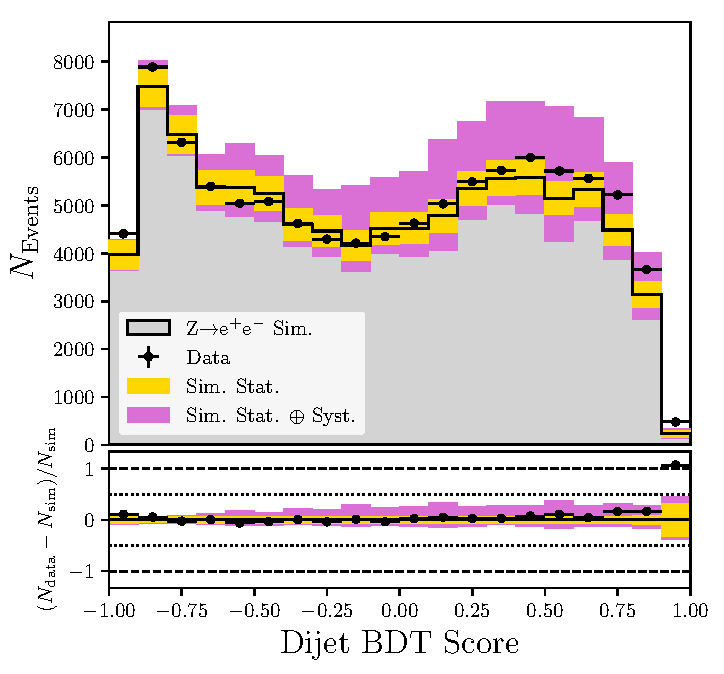
\includegraphics[width=0.49\textwidth]{figures/event_selection/dijet_BDT_zee_PS.pdf}
        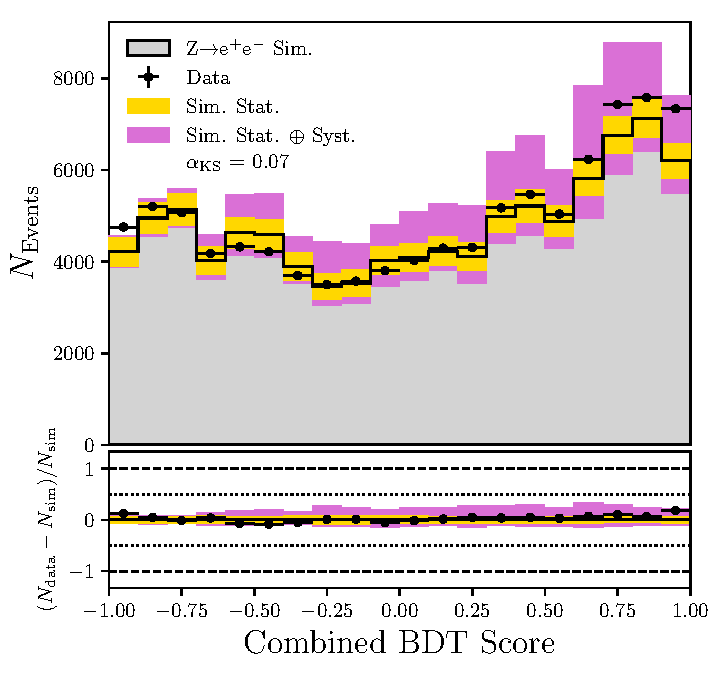
\includegraphics[width=0.49\textwidth]{figures/event_selection/combined_BDT_zee_PS.pdf}
    \end{center}
    \caption{Zee validation plots for the BDTs}
    \label{fig:event_categorisation:zee_bdt_score_validation}
\end{figure}


\begin{figure}[h!]
    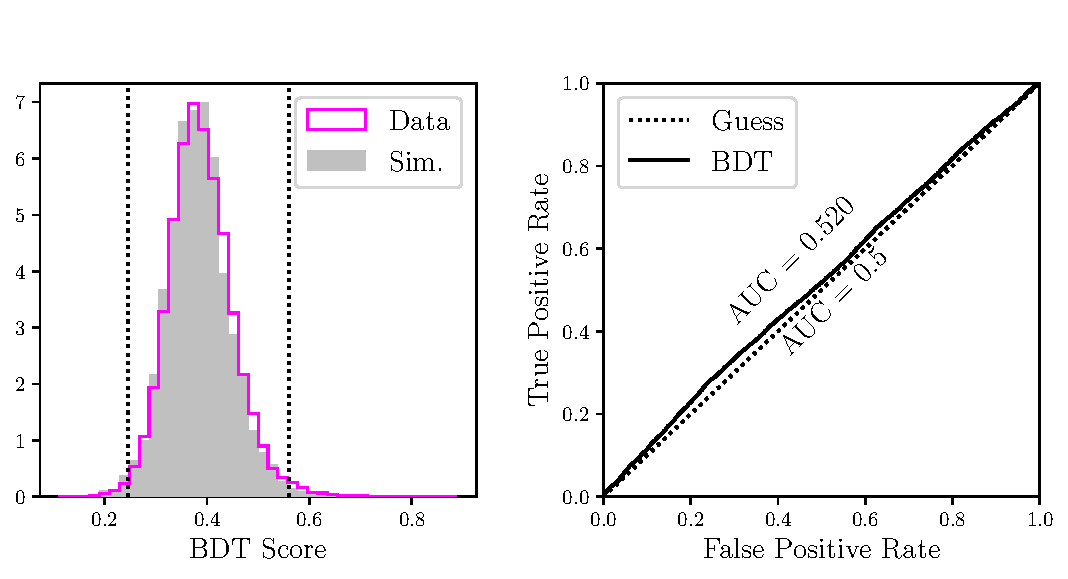
\includegraphics[width=0.75\textwidth]{figures/event_selection/eng_feature_ROC_Zee_BDT.pdf}
    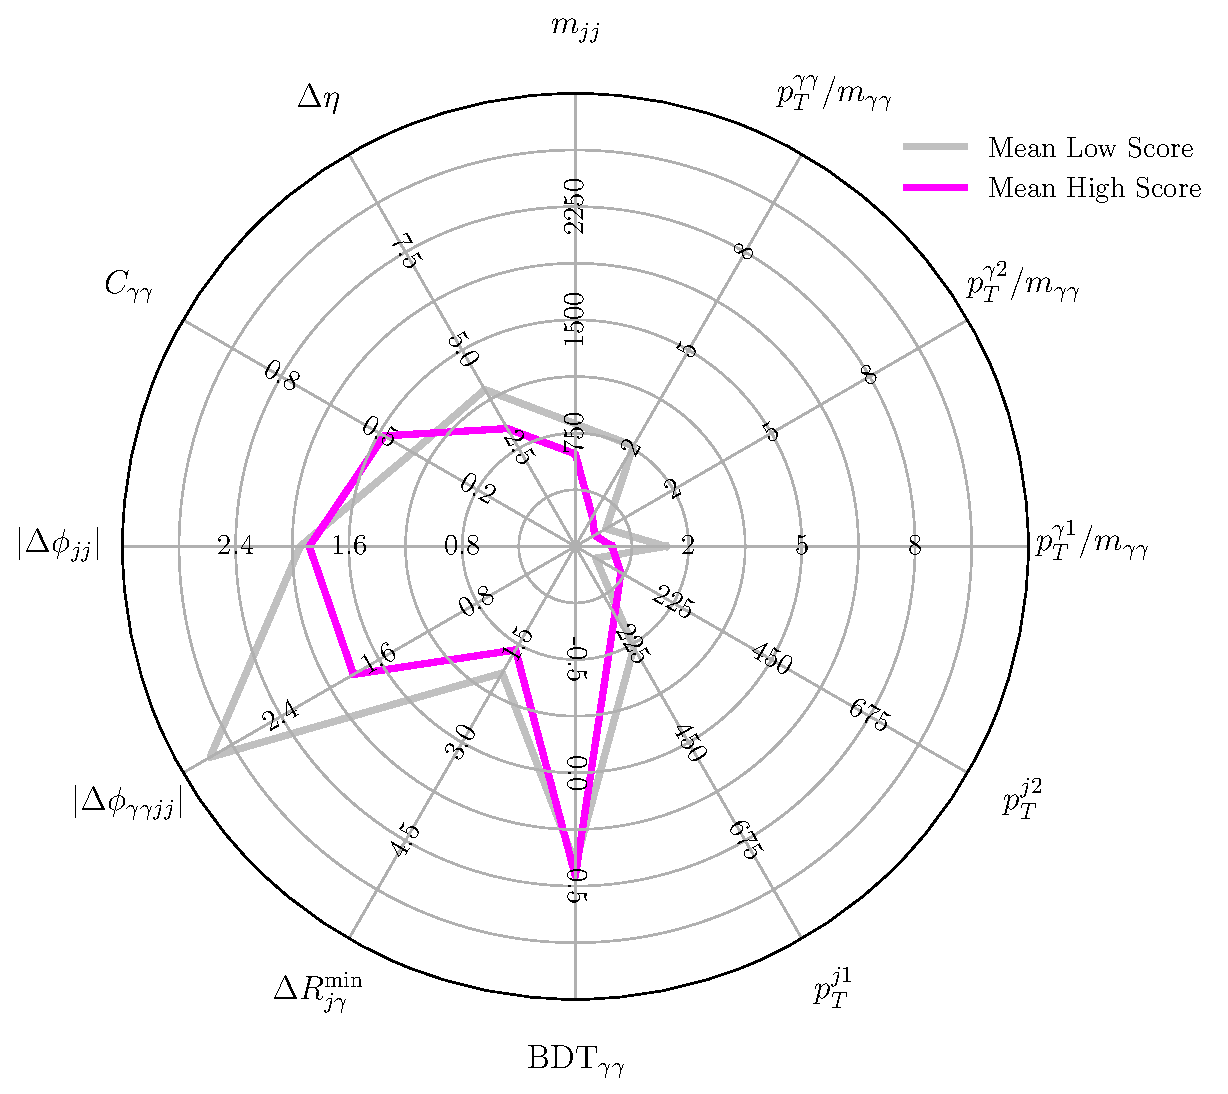
\includegraphics[width=0.75\textwidth]{figures/event_selection/eng_feature_radar_Zee_BDT.pdf}
    \caption{Joint distribution study with BDT in Zee control region}
    \label{fig:event_categorisation:zee_bdt_validation}
\end{figure}

\begin{figure}[h!]
    \begin{center}
        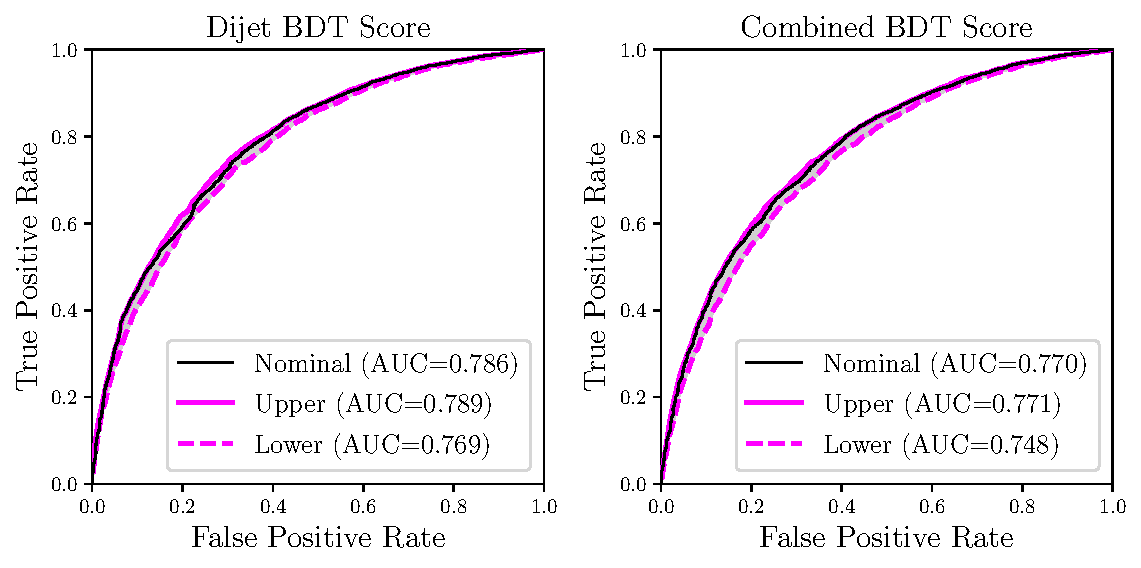
\includegraphics[width=0.95\textwidth]{figures/event_selection/psvar_ROCs_PS.pdf}
    \end{center}
    \caption{PS/Tune variants}
    \label{fig:event_categorisation:ps_variant_validation}
\end{figure}





\subsection{Single BDT Model}
Really it should be a single step. This was developed on old technology with the old cuts. The ID cut does the job of the combined BDT now, and it just replicates the dijet BDT score. Conclusion is that the combined BDT is useless and the diphoton score should just be added to the set of dijet BDT input features. This gives the same performance and will be what we use to compare with the DCNN. 

\begin{figure}[h!]
    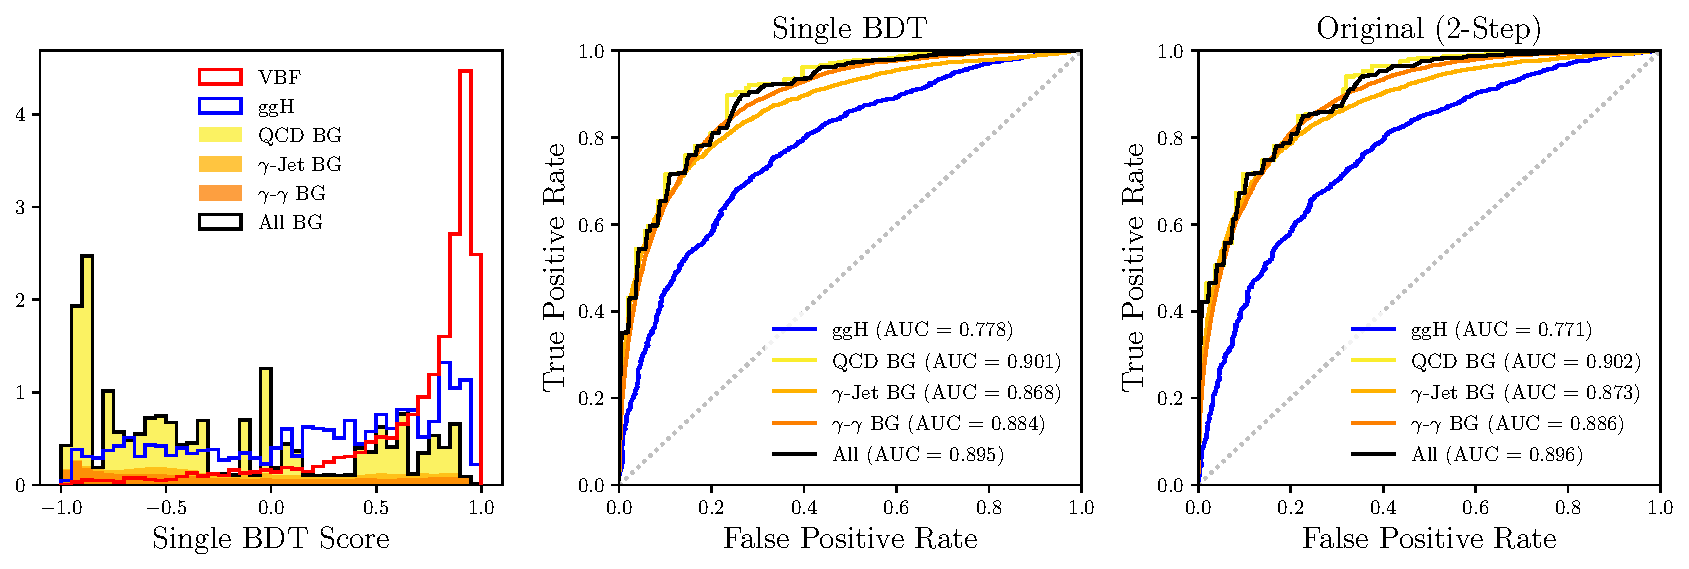
\includegraphics[width=0.99\textwidth]{figures/event_selection/dijet_BDT_PS_unw.pdf}
    \caption{Single BDT performance}
    \label{fig:event_categorisation:single_BDT}
\end{figure}











\section{VBF Tag with a Dense Convolutional Neural Network}
Introduction, mention that the selection is the same, objectives and motivation for the new tag
2016 underperforms with ggH. ggH is a harder problem to solve. Need to go beyoned kinematics. Use jet structure.
A general way of representing this substructure is images. Dense CNNs are good at classifying images. 
We can use a dense CNN to form performant features without the need for human intervention. 

The objective of the new tag is to use jet images and a dense CNN to enhance VBF signal extraction, especially VBF vs Gluon Fusion discrimination. 
We will also introduce cost-sensitivity to the ML problem which has been done in an approximate unsystematic fashion before

Because the problem of building the model is so complex we'll use optimisation to do it for us. 

We'll also use a few techniques to figure out what sort of features it has build. Is it able to pick up on colour connection etc?

\subsection{Jet Images}
The spatial distribution and properties of a jet's constituent particles contain important discriminating information about the originating parton. 
An image is a natural way of representing this information with the spatial distribution represented by the arrangement of pixel values and the channels of the image representing properties such as charged particle $p_{T}$ in the pixel region.

\subsubsection{Formulation}
The image formulation used in this thesis is of two three-channel images stacked in the channels dimension to produce a $n\times{}n\times{}6$ dijet image.
The three channels are the following: $p_T$ deposition of charged candidates, $p_T$ deposition of neutral candidates, and particle multiplicity.
The space that the pixels correspond to is the space of particle displacements in pseudorapidity and azimuthal angle from the jet axis $(\Delta\eta,\Delta\phi)$,
\begin{equation}
    \begin{split}
        \Delta\eta =& \eta_{p} - \eta_{j} \\ 
        \Delta\phi =& \phi_{p} - \phi_{j} \\
    \end{split}
    \label{eq:event_categorisation:pixel_coords}
\end{equation}
where subscript $p$ denotes a constituent particle and $j$ denotes the jet. 
The pixels themselves are not a recilinear grid in $(\Delta\eta,\Delta\phi)$, but are evenly-spaced in the polar coordinates 
\begin{equation}
    \begin{split}
        \Delta{R} =& \sqrt{\Delta\eta^2 + \Delta\phi^2} \\
        \varphi   =& \mathrm{tan}(\Delta\phi/\Delta\eta) \\
    \end{split}
    \label{eq:event_categorisation:pixel_coords}
\end{equation}
These have been rotated by half a pixel in $\varphi$ so that the $(\Delta\eta,\Delta\phi)$ axes line up with the centres of a row of pixels rather than the boundary between them. 
Finally, the images are normalised such that the sum of the $p_T$-based channels equal one, and the sum of the individual multiplicity channels equal one. 
The image formulation is summarised in Figure \ref{fig:event_categorisation:jet_image}.

These images are different in their formulation and behaviour compared to a typical image.
Firstly, they are sparse with only a fraction of the pixels ever non-zero in any one image. 
Secondly, assumptions about local correlations between pixels do not apply: two adjacent red pixels would mean two adjacent particles. Max pooling will simply pick the higher valued pixel during downsampling and information about the second particle will be lost. 
Thirdly, in the rectilinear image which is seen by the network (bottom right of Figure \ref{fig:event_categorisation:jet_image}) there is a periodic boundary condition where the top pixels wrap around to the bottom ones. When convolution operations are performed on these images the padding must be periodic in the vertical direction ($\varphi$ direction).

\newpage
\begin{figure}[h!]
    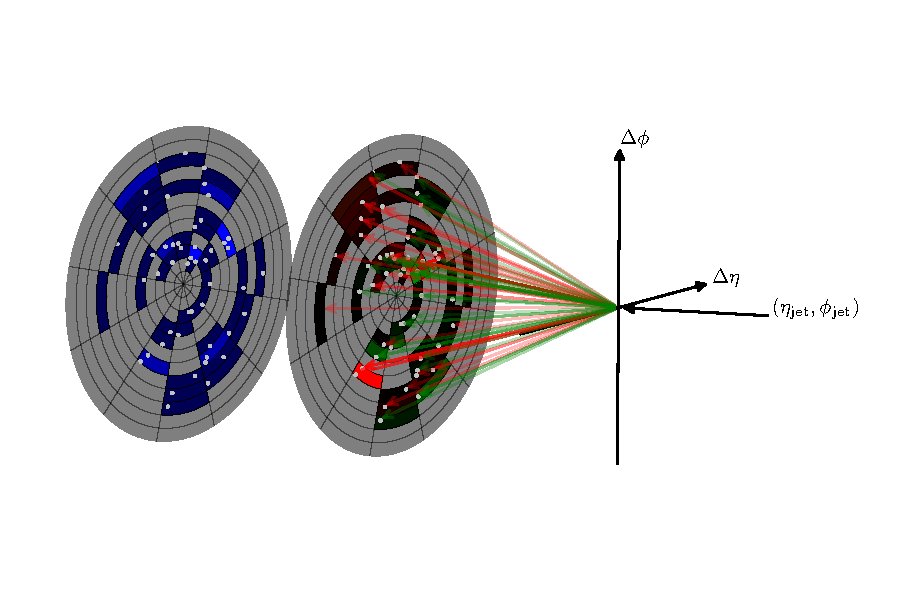
\includegraphics[width=\textwidth]{figures/event_selection/jet_diagram_RGB.pdf}
    \begin{center}
        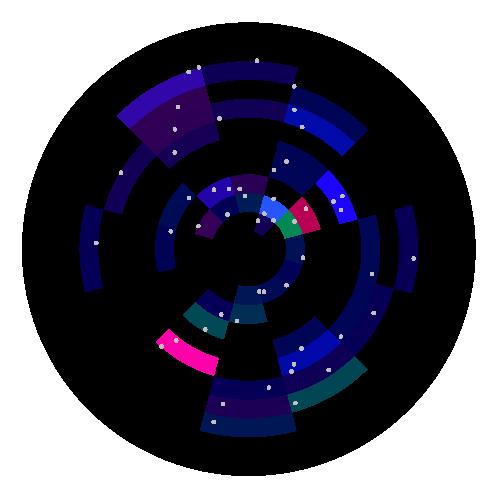
\includegraphics[width=0.49\textwidth]{figures/event_selection/full_image_polar.pdf}
        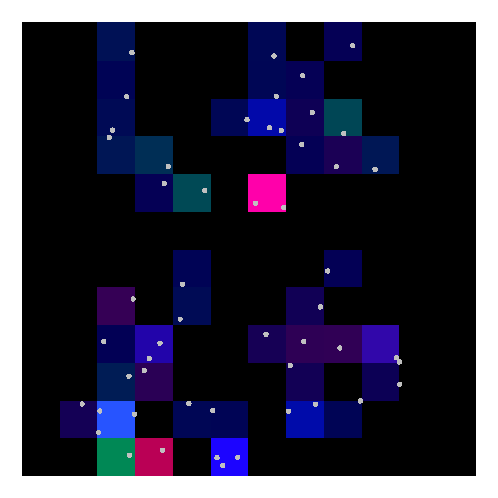
\includegraphics[width=0.49\textwidth]{figures/event_selection/full_image_rect.pdf}
    \end{center}
    \caption{\textbf{Top:} 
             construction of single-jet image from jet constituents. Arrows correspond to individial PF candidates where red arrows are charged, green are neutral and the opacity corresponds to $p_{T}$.
             The red channel measures charged candidate $p_T$ deposition in each pixel, 
             the green channel is neutral charged candidates $p_T$ deposition, 
             and the blue channel is the number of candidates in each pixel (multiplicity). 
             Multiplicity channel is drawn separately so the charged and neutral channels can be seen clearly. Black pixels are lightened to show coloured pixels more clearly.\\
             \textbf{Bottom:} 
             the final image with all the channels together.}
    \label{fig:event_categorisation:jet_image}
\end{figure}


\subsubsection{Image Dataset}
Mean images and decompositions for structure, coarse structure of forward regions
\begin{figure}[h!]
    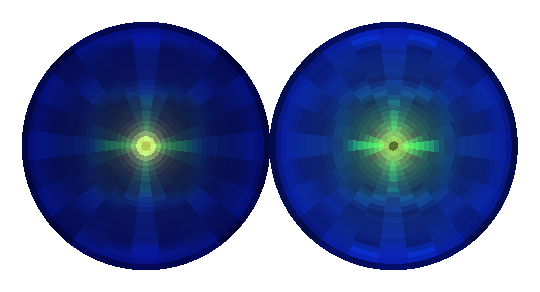
\includegraphics[width=0.75\textwidth]{figures/event_selection/mean_vbf_PS_uw.pdf}
    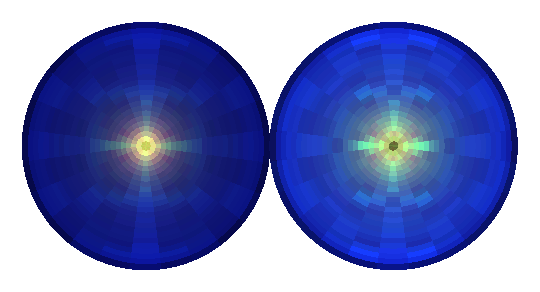
\includegraphics[width=0.75\textwidth]{figures/event_selection/mean_ggh_PS_uw.pdf}
    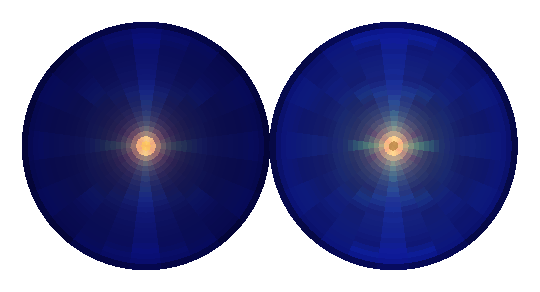
\includegraphics[width=0.75\textwidth]{figures/event_selection/mean_bkg_PS_uw.pdf}
    \caption{Mean images}
    \label{fig:event_categorisation:mean_jet_image}
\end{figure}



\subsection{Model Design}

The overall structure of the model can be considered to built from three main parts:
\begin{itemize}[leftmargin=.5in,noitemsep]
    \item \textbf{Convolutional section} for learning dijet substructure features from dijet images.
    \item \textbf{Merge section} for processing and integrating engineered kinematic features with learned features from the convolutional section.
    \item \textbf{Main discriminant} fully-connected layers for integrating all information and producing the class logits.
\end{itemize}


The convolutional section consists of a `spread layer' followed by three dense blocks each of which are followed by transition units.

The spread layer is a depthwise convolution layer which produces $N$-many featuremaps for each channel where the filters do not mix the image channels. 
For each channel's associated feature maps half of them have their values evenly permuted in the vertical direction, this corresponds to a rotation by $\pi$ in the polar image.
The function of this layer is to spread out the sparse image into a collection of featuremaps which correspond to simple local spatial configurations of pixels such as radial or angular bands of deposition. 
The interleaved rotations of this layer's output featuremaps allows for the comparison of pixels opposite each other around the jet axis much earlier in the network.  
This layer gives two hyperparameters to the model: the filter size and the number of features per input channel.

The dense blocks construct increasingly higher-level featuremaps, and the transition units will combine feature maps for feature reduction as well as downsampling with average pooling to avoid information loss associated with max pooling mentioned before.  
The structure of each of these parts is tuneable, and therefore gives another twelve hyperparameters to the model: three from each dense block and one from each transition unit. 

The merge section consists of a set of fully-connected layers with the first one after the initial input a different size to the others, this is then concatenated with the output of the convolutional part.
The function of this section is to embed the engineered features in a higher-dimensional space, form them into a vector the same size as the convolutional section output, and then combine them together with the jet structure features. This section has three hyperparameters: the size of the hidden layers, the number of layers, and the size of the first hidden layer relative to the others. 


The main discriminant consists of a sequence of fully-connected layers which take the full vector of concatenated features as input and produce three class logits which correspond to the VBF, ggH, and background process classes. 
These logits are then mapped to class probabilities by a softmax function, the VBF class probability is then used to define tag categories. 

\subsection{Loss and Regularization}
(Weights and their interpretation as cost)
(Cost sensitivity: intra class and inter class costs)

Cost explaination, how the previous one tried to do costing with the ggH being left out of the combined BDT training. 

The loss function is a cost-sensitive version of cross entropy from (ref)
\begin{equation}
    L_i = -\log\left(\frac{\xi_{pp}e^{o^{i}_{p}}}{\sum_{j=0}^{3}\xi_{pj}e^{o^{i}_{j}}}\right)
\end{equation} 
where $i$ enumerates the events of the minibatch, $o_j$ is the logit of class $j$, $p$ is the true class index of the event, and $\xi$ is the cost matrix which encodes misclassification costs
\begin{equation}
    \xi = \begin{pmatrix}
        c_{\mathrm{BG}} & c_{\mathrm{BG}/\mathrm{ggH}} & c_{\mathrm{BG}/\mathrm{VBF}} \\
        c_{\mathrm{BG}/\mathrm{ggH}} & c_{\mathrm{ggH}} & c_{\mathrm{ggH}/\mathrm{VBF}} \\
        c_{\mathrm{BG}/\mathrm{VBF}} & c_{\mathrm{VBF}/\mathrm{ggH}} & c_{\mathrm{VBF}} \\
    \end{pmatrix}
\end{equation}
where each element $c$ is a real number belonging to the interval $(0,1]$. A cost of zero assigns

The loss over the entire minibatch is expressed as a weighted sum of events,
\begin{equation}
    L = \frac{1}{\sum_{j=0}^{N}w_{j}}\sum_{i=0}^{N}w_{i}L_{i}
\end{equation} 
where $N$ is the number of elements in the minibatch, and $w_i$ is the weight of event $i$.

These event weights are handled as follows


(The regularisation)
The model is regularised with $L_2$ throughout, but with separate values for the different sections. There is also dropout applied to the fully-connected layers during training. 
Dropout is not applied to the convolutional part. 



The loss function used is a weighted version of cross entropy where the loss over the minibatch is a weighted mean. For each batch the optimiser will descend the weighted mean of the gradients for each example in the minibatch. The weights are normalised per class so each class has the same total weight, but the shape of their distribution is preserved.  


\subsection{Data Preprocessing and Training}
The optimisation uses stochastic gradient descent with Nesterov momentum and learning rate decay. This is found (ref) to give better generalisation than algorithms with adaptive per-parameter learning rates such as Adam. 

All of the input features are preprocessed with mean-subtraction and division by their standard deviation. The means and standard deviations are calculated from the training set and these values are applied to the validation and test sets as well as the training set. 
The the training data are augmented by randomly reflecting the images in the $\Delta\eta$ and $\Delta\phi$ directions during training. 



\subsection{Neural Architecture Search}
Network architecture optimisation

The final model post-opt 



\subsection{Regularization}
Now control the model capactity with regularisation. 


\subsection{Final Model Performance and Categorisation}
The performance of the final model with comparison to the legacy


\subsection{Learned Features Interpretation}
We would like to figure out what sort of features the convolutional section is forming. There are three approaches we will explore here: maximally activating images from the dataset, image occlusion studies, and the production of maximally activating images using stochastic gradient descent (deep dreams).  


\subsection{Validation}
Zee validation of the score plus the data/sim training to tell the images apart and feature vis of the differences. Comparison to BDT-based tag. 


\section{Untagged}
If the candidate does not receive a tag it is conisdered for the untagged categories which make a selection diphoton BDT score. These categories mostly consist of gluon fusion events. 


